\documentclass{article}
\usepackage{graphicx} 
\usepackage{authblk}   
\usepackage[margin=1in]{geometry} 
\usepackage[font=small,skip=4pt]{caption}
\usepackage{float}
\usepackage{microtype}
\usepackage[hyphens]{url}
\usepackage[
  backend=biber,
  style=numeric,    
  sorting=none
]{biblatex}
\addbibresource{references.bib}   
\providecommand{\citealp}[1]{\cite{#1}}

\usepackage{hyperref}   % load last


\title{A question-and-answer classification dataset for borderline personality disorder screening}

\begin{document}
\author[1]{Shadman Shafeen Khan\thanks{shadmanshafeen@gmail.com}}
\author[1]{Muntasir Hasan Porag\thanks{hasanmuntasir257@gmail.com}}
\author[1]{Nusrat Sharmin\thanks{@gmail.com}}
\author[1]{Md.\ Mahbubur Rahman\thanks{@gmail.com}}
\date{October 2025}

\affil[1]{Department of Computer Science and Engineering, Military Institute of Science and Technology, Mirpur Cantonment, Dhaka 1216, Bangladesh}

\maketitle
\abstract{Borderline personality disorder (BPD) is a serious mental health condition marked by unstable emotions, identity, and relationships, and it carries a high risk of self-harm and suicide. Automated screening could help identify people who need clinical attention, but progress is held back by a lack of reliable text data. Most existing mental health datasets are scraped from social media, where labels are self-reported, demographic coverage is narrow, and responses are not tied to any diagnostic framework. This paper presents BPDQAC, a question-and-answer classification dataset developed for BPD screening. It contains 3,258 question-answer pairs from 362 consenting participants, collected using a 14-question instrument aligned with DSM-5 criteria. Nine open-ended questions target Criterion A symptoms, and five yes/no questions cover Criteria B through F. Each pair was labelled as Normal, BPD-indicative, or Inconclusive by a psychiatrist, a clinical psychologist, and a trained counselor, with semi-supervised label propagation extending expert judgement across the full dataset. Eight transformer models were then fine-tuned on the data to establish baseline performance, and XLNet achieved the strongest result with a weighted F1-score of 0.862. The findings show that BPDQAC supports reliable supervised learning and offers a clinically grounded resource for research on automated BPD screening.
}
\section{Introduction}


Borderline personality disorder is a severe mental health condition defined by a consistent pattern of unstable relationships, self-perception, and emotions, along with impulsive behavior that typically emerges in early adulthood and occurs across different situations.
The estimated median prevalence of borderline personality disorder in the general population is 1.6\%, though it could reach as high as 5.9\%. In primary care settings, the prevalence is approximately 6\%, while it rises to around 10\% in outpatient mental health clinics and reaches about 20\% in psychiatric inpatient populations \cite{dsm}.
Follow-up studies have indicated that suicide occurs in as many as 10\% of cases involving borderline personality disorder \citealp{paris2001,stone1990}. Research suggests that between 40\% and 85\% of individuals with borderline personality disorder engage in suicide attempts, which are often recurrent, with an average of three attempts per individual. Moreover, self-harm is prevalent among individuals with borderline personality disorder, affecting 50 to 80\% of cases, and is often repetitive, with more than 41\% of patients engaging in over 50 instances of self-mutilation \cite{oumaya2008}.
The diagnosis of BPD typically relies on in-person interviews with licensed mental health professionals, and the utilization of Likert Scales or Dichotomous Questionnaires like the McLean Screening Instrument for Borderline Personality Disorder (MSI-BPD) \cite{zanarini2003}. \\

However, mental health is often neglected in developing countries with limited resources, and mental illnesses like BPD often remain undiagnosed. For example, a recent study reports that about 90\% of people with mental health conditions in Bangladesh do not seek or receive treatment \cite{huque2025}.\\

In recent years, the application of Artificial Intelligence in mental health diagnostics \cite{sr2024, lawrence2024, perlis2024} has yielded encouraging outcomes. Research has employed a variety of methodologies to identify individuals affected by borderline personality disorder \cite{lahnakoski2024, arango2024, nazari2024}.
However, research highlights a significant lack of availability of reliable, expert-annotated text datasets related to borderline personality disorder and other mental health conditions \cite{mocnik2024, zhang2022}.

Several datasets pertinent to borderline personality disorder have been presented in the literature. For instance, Khan et al. \cite{khan2023} measured BPD symptoms using the McLean Screening Instrument for BPD (MSI-BPD) and depression using the Patient Health Questionnaire-9 \cite{kroenke1999} through an online questionnaire that includes demographics and self-reported BPD/depression scores.

While these datasets have facilitated the application of AI tools in automating the identification of borderline personality disorder (BPD), they remain insufficient for training AI models to accurately screen patients. Notably, the majority of BPD-related datasets are derived from social media scraping, which lacks the clinical rigor necessary for diagnosing BPD or other mental illnesses in individuals. 

This study addresses the aforementioned gaps by presenting a dataset comprising expert-annotated question-answer pairs. This dataset can be utilized to train AI models to screen individuals for Borderline Personality Disorder (BPD) by simulating interviews conducted by mental health professionals. The inclusion of nine open-ended questions for Criterion A and five dichotomous questions for Criteria B-F provides a structured framework to assess whether an individual's responses correspond to the diagnostic criteria for BPD. It is important to note that each question has been meticulously crafted by mental health experts in accordance with specific diagnostic criteria for Borderline Personality Disorder (BPD), and therefore, the corresponding responses can serve as indicators for assessing whether an individual meets the criteria for BPD.


\section{Literature Review}\label{sec1}

% The application of natural language processing (NLP) to mental health detection has evolved substantially over the past decade, progressing from traditional machine learning approaches to sophisticated transformer-based architectures. This section traces that evolution, examines persistent limitations in existing datasets and methodologies, and identifies the specific gap that motivates the present study.




The application of natural language processing (NLP) to mental health detection has evolved substantially over the past decade. The filed has progressed from traditional machine learning appraches to sophisticated transformer-based architectures. This section traces back the evolution and highlights existing limitation in the current methodologies and datasets.
















% the application of natural language












\subsection{Early Approaches: Traditional Machine Learning on Social Media}

% Early work in computational mental health detection relied primarily on social media platforms as data sources and employed traditional machine learning classifiers. Singh et al. \cite{singh2020framework} developed a framework for detecting antisocial behavior on Twitter using NLP preprocessing techniques combined with classifiers such as Logistic Regression, Support Vector Machines, Naive Bayes, and Decision Trees. This approach established a pattern that would dominate the field: leveraging publicly available social media text to identify psychological indicators. A comprehensive meta-analysis by Harrigian et al. \cite{harrigian2021state} catalogued 102 social media datasets used in mental health research, revealing that Twitter and Reddit were the most common platforms, while depression and suicidal ideation were the most frequently studied conditions. This early foundation demonstrated that language patterns in informal online text could signal mental health states, though the reliance on self-reported labels and platform-specific data introduced significant limitations.







%human

Early work in mental health detection mostly relied on social media platform as their primary data sources. These studeies explored traditional Machine learning classifiers before transformer-based model were introduced. Sign et al. \cite{singh2020framework} developed an antisocial behavior classifier on Twitter using NLP preprocessing techniques combined with traditional Machine learning classifiers, which includes Logistic Regression, Support Vector Machines, Naive Bayes and Decision Trees. This approach introduced a new area of research that has dominated the field since: leveraging publicly available social media data to identify psychological indicators. A comprehensive meta-analysis by Harrigian et al. \cite{harrigian2021state} catalogued 102 social media datasets used in mental health research. Their finding revealed that Twitter and Reddit were the most common platforms for data collection, while depression and suicidal ideation were the most frequently studied mental health states. Here the main limitations were self-reported labels, which introduce reliability issue and platform specific data, which raises concerns about generalizability. Here the main limitation were self-reported labels, platform specific data and limited symentic learning capability of the traditional ml models, which introduces reliability issue, limited generalizability and poor performance. 


















\subsection{Evolution to Deep Learning and Transformers}

% The transition from traditional machine learning to deep learning architectures marked a significant improvement in detection performance. Dinu and Moldovan \cite{dinu2021automatic} applied transformer models including BERT, RoBERTa, and XLNet to classify mental illnesses from general Reddit posts, achieving up to 81\% accuracy. Their work demonstrated that mental health conditions could be detected even from text not explicitly discussing mental health topics. Jiang et al. \cite{jiang-etal-2020-detection} constructed a large-scale Reddit dataset comprising 17.5 million posts from users with eight different mental health disorders, employing deep contextualized BERT representations for classification. Their findings showed that user-level classification significantly outperformed post-level classification. In the domain of suicidal ideation detection, Haque et al. \cite{suicidalideationtransformers2020} compared multiple transformer architectures and found that RoBERTa achieved 95.21\% accuracy on Reddit SuicideWatch data. Ellouze and Belguith \cite{ellouze2022deep} explored deep learning architectures combining CNN and LSTM layers for personality disorder detection, demonstrating the potential of hybrid approaches. Despite these advances in model performance, the fundamental reliance on social media data and multi-class generalization remained unchanged.












The transition from traditional machine learning to complex deep learning architectures marked a significant imporvement in detection performance. Dinu and Moldovan el al. \cite{dinu2021automatic} applied transfoemer models including BERT, RoBERTa and XLNet to classify mental health conditions using generaal Reddit posts. Their approach achieved up to 81\% accuracy, Demonstrating that mental helth conidtions could be detected even from text not just explicity discussing mental health topics. another study by Jiang et al. \cite{jiang-etal-2020-detection} where they constructed a user-specific Reddit dataset consisting 17.5 million posts from users with eight distinct mental health disorders employed with contextualized BERT representations for classification. Their findings showed that user-level classification significantly outperformed post-level classification. In the domain of suicidal ideation detection, Haque et al. \cite{suicidalideationtransformers2020} compared multiple transformer architectures and found that RoBERTa achieved 95.21\% accuracy on Reddit SuicideWatch dataset. Ellouze and Belguith \cite{ellouze2022deep} explored deep learning architectures combining CNN and LSTM layers for personality disorder detection, demonstrating the potential of hybrid approaches. Despite these advancement in model's performance, the fundamental reliance on social media data and limited generalization remained unchanged.
















\subsection{Domain-Specific Mental Health Language Models}

% Recognizing that general-purpose language models might not capture the nuances of mental health discourse, researchers developed domain-specific models. Vajre et al. \cite{vajre2021psychbert} introduced PsychBERT, a BERT model pretrained on biomedical mental health literature and social media text, achieving an F1-score of 0.98 for detecting mental health-related content. Yang et al. \cite{yang2024mentallama} proposed MentaLLaMA, an instruction-tuned large language model trained on the IMHI dataset comprising 105,000 samples, which provided interpretable explanations alongside predictions. Xu et al. \cite{xu2024mental} demonstrated that instruction fine-tuning significantly improves large language model performance on mental health prediction tasks. Martinez-Castano et al. \cite{martinez2022early} applied BERT-based transformers to early detection of self-harm, achieving 91.3\% precision. These domain-specific approaches improved both accuracy and interpretability, yet the underlying training data remained predominantly social media-based, limiting clinical applicability.




% human


Recognizing that general-purpose language models might not undrestand the nuances of mental health discourse, researchers developed domain-specific models. Vajre et al. \cite{vajre2021psychbert} introduced PsychBERT, a specialized BERT model pretrained on biomedical mental health literature and social media text. PsychBERT achieved an F1-score of .98 for detecting mental health condition. MentaLLaMA proposed by Yang el al. \cite{yang2024mentallama}, an instruction-tuned large language model trained on the IMHI dataset consiting 105,000 samples. MentaLLaMA provided interpretable explainability alongside predictions. Xu et al.\cite{xu2024mental} also demonstrated that instruction-tuning significantly imporved large language model performance on mental health detection task. another study by Martinez-Castano et al.\cite{martinez2022early} applied BERT-based transformers to early detection of self-harm, achieving 91.3\% precision. These domain-specific approaches further improved performance and  introduced interpretability. However, the underlying training data still remained predominantly social media-based, limiting clinical applicability.
























\subsection{Survey Findings and Critical Dataset Limitations}

% Several comprehensive reviews have synthesized the state of mental health NLP research and identified systemic limitations. Montejo-Raez et al. \cite{montejo2024survey} surveyed the literature and found that depression was the most studied condition with 249 publications, while noting that English-language dominance, privacy concerns, and social media bias remained unresolved challenges. Zhang et al. \cite{zhang2022natural} conducted a narrative review of 399 articles and reported that 81\% of studies relied on social media data, expert-annotated datasets were scarce, and clinical validation of NLP systems was rare. Greco et al. \cite{greco2023transformer} confirmed transformer dominance in recent work while highlighting data quality as a critical bottleneck.





Several comprehensive reviews have summarized the progress of mental health NLP  research and highlighted important limitation in the field. Montejo-Raez el al. \cite{montejo2024survey} surveyed the literature and found that depression was the most frequently studied mental health condition with 249 publications. They also noted that English-language dominance, privacy concerns and social media bias remained unresolved challenges. A narrative review of 399 articles conducted by  Zhang el al.\cite{zhang2022natural} found that 81\% of the studies relied on scoial media data, expert annotated datasets were scarce and clinical vlaidation of NLP systems were rare. Greco et al. \cite{greco2023transformer} confirmed transformer dominance in recent work while highlighting data quality as a critical bottleneck.
















% These reviews expose fundamental problems with social media-based approaches. First, demographic bias is inherent in platform populations; Reddit users, for instance, skew toward young male individuals \cite{dinu2021automatic}. Second, privacy and ethical concerns arise when analyzing users without informed consent \cite{montejo2024survey}. Third, labels derived from self-reported diagnoses rather than clinical assessment introduce noise and uncertainty \cite{jiang-etal-2020-detection}. Fourth, prediction scores are often poorly calibrated for actual clinical risk assessment \cite{jiang-etal-2020-detection}. Finally, data accessibility remains limited, with only 35 of 102 identified datasets publicly available \cite{harrigian2021state}. These limitations collectively undermine the clinical applicability of social media-based mental health detection systems.







These reviews highlighted the fundamental limitations with  social media-based approaches. Firstly, social media dataset often contain demographic bias because platform users are mostly young and they dont represent the general population. For example, a study by Dinu et al \cite{dinu2021automatic} showed Reddit users tend to be young and predominantly male. Secondly, privacy and ethical concerns arise when user specific content is analyzed without their direct consent \cite{montejo2024survey}. Thirdly, many dataset rely on self-reported labels rather than clinicla assesment, which introduce noise and uncertainty in data \cite{jiang-etal-2020-detection}. Fourthly, prediction scores from these systems are often not well calibrated for real world clinical risk assessment \cite{jiang-etal-2020-detection}. Finally, data accessibility remains limited, only 35 of 102 identified datasets publicly available \cite{harrigian2021state}. Together, these limitations reduce the clinical applicability of mental health detection systems trained primarily on social media data.
























\subsection{Personality Disorder Detection}

% Research on personality disorders emerged as a distinct subfield within computational mental health. Jain et al. \cite{jain2024text} developed text classification models for multi-class personality disorder identification using BERT, achieving 74.7\% accuracy on their PD-TXT dataset. Ellouze and Belguith \cite{ellouze2022hybrid} proposed a hybrid architecture combining CNN, BiLSTM, and SVM, achieving 84\% F1-score for personality disorder detection from tweets. Ellouze and Belguith \cite{ellouze2024artificial} provided a comprehensive survey of AI applications for personality traits and disorders in social media, documenting the shift from traditional machine learning to deep learning approaches. Baqasah \cite{baqasah2024personality} applied LSTM-based deep learning to social media analysis, achieving 89\% accuracy in detecting personality disorders. While these studies expanded beyond general mental health detection to personality-specific classification, they maintained the pattern of relying on social media data and performing broad multi-class categorization rather than focusing on individual disorders.







Research on personality disorders has become a separate subdomain in computational mental health research. Jain et al.\cite{jain2024} developed text classificaiton models for multi-class personality disorder identification using BERT, Achieving 74.7\% accuracy on their PD-TXT dataset. Ellouze and belguith \cite{ellouze2022hybrid} proposed a hybrid architecture combining CNN, BiLSTM, and SVM, achieving an F1-score of 84\% for personality disorder detection from tweets. In a later survey, Ellouze and Belguith \cite{ellouze2024artificial} review AI-Based appraches for detecting personality traints and disorders in social media data. They also highlighted the shift from traditional machine learning to deep learning appraches. Baqasah et al.\cite{baqasah2024personality} applied LSTM-based deep leaning model to social media data analysis, achieving 89\% in detecting personality disorders. While these studies expanded beyond general mental health detection to personality specific classificaiton, they maintained their reliance on social media data. Most of These studies focuese on performing broad multi-class classification rather than focusing on specific disorders.








\subsection{BPD-Specific Computational Work}

% Compared with depression, anxiety, or general personality disorder classification, computational studies specifically targeting borderline personality disorder remain limited. Khazbak et al. \cite{khazbak2021mindtime} developed MindTime, a diary application that analyzed users' daily notes on events, experiences, thoughts, and emotions to detect BPD symptoms. Using SVM and LSTM classifiers, they achieved user accuracy of 90.1\% and 91\% respectively. However, this approach relied on personal diary entries rather than structured clinical assessment. Wang et al. \cite{wang2020learning} used language and speech features from non-clinical interviews to distinguish between bipolar disorder, BPD, and healthy controls, achieving an AUROC of 0.733 for BPD detection. Their dataset comprised only 50 interviews, limiting generalizability. These studies demonstrate that BPD can be approached computationally, yet neither employs expert-annotated responses to structured diagnostic questions aligned with clinical criteria.









In compare to depression, anxiety, or general personality disorder classification, computational studies specifically targeting borderline personality disorder remain limited. Khazbak et al. \cite{khazbak2021mindtime} developed MindTime, a diary application that analyzed users' daily notes on events, experiences, thoughts and emotions to detect BPD symptoms. Using SVM and LSTM classifers they achieved an accuracy of 90.1\% and 91\% respectively using user specific data. However, the key limitation of the study was its reliance on personal diary entries rather than structure clinical assessment. Another study by Wang  el al. \cite{wang2020learning} used language and speech features from non-clinical interviews to distinguish between bipolar disorder(BPD), and healthy behavior. Their apprach achieved an AUROC of 0.733 for BPD detection. Their dataset comprised only 50 interviews, limiting generalizability. These studies demonstrate that BPD can be approached computationally, yet neither of the study used structured diagnostic questions aligned with clinical criteria along with expert-annotated response.














\subsection{Question-Answering in Mental Health: A Different Purpose}

Question-answering approaches have appeared in mental health AI, but with fundamentally different objectives than patient screening. Guo et al. \cite{guo2021mental} developed a mental health question-answering system combining BERT with knowledge graph technology, designed to answer users' mental health questions rather than to assess their psychological state. Racha et al. \cite{racha2025mhqa} introduced the MHQA dataset containing approximately 58,000 question-answer pairs for benchmarking language model knowledge on mental health topics related to anxiety, depression, trauma, and OCD. This dataset evaluates whether models possess factual knowledge about mental health conditions, not whether they can screen individuals based on their responses to diagnostic questions. These efforts move toward question-answer formats but do not address how an individual's own responses to structured questions can be classified for disorder-specific screening.





















\subsection{Research Gap}

The preceding review reveals a clear gap in the literature. First, the overwhelming majority of mental health NLP research relies on social media data, which is fundamentally inadequate for clinical screening due to consent issues, demographic bias, noisy labels, and lack of clinical validation \cite{zhang2022natural}. Second, most work focuses on generalized multi-class classification across several mental health conditions rather than specialized screening for individual disorders \cite{montejo2024survey}. Third, BPD-specific computational research is extremely limited, confined to diary-based \cite{khazbak2021mindtime} or interview-based \cite{wang2020learning} approaches that do not utilize expert-annotated responses to structured diagnostic questions. Fourth, existing question-answering work in mental health addresses knowledge retrieval and model benchmarking \cite{guo2021mental, racha2025mhqa}, not patient screening through response classification.

Critically, this gap contrasts with actual clinical practice: psychiatrists and psychologists diagnose BPD through structured, criterion-based questioning aligned with DSM-5, not through analysis of social media posts. No existing dataset provides expert-annotated question-answer pairs specifically designed for BPD screening where individuals' responses to diagnostic questions are labeled according to whether they indicate the presence of BPD symptoms. This study addresses that gap by introducing BPDQAC, a specialized question-answer classification dataset created in collaboration with mental health experts and aligned with clinical diagnostic criteria.



























\section{Dataset}\label{sec2}
This section describes the construction of BPDQAC, including questionnaire formulation, response collection, data cleaning, annotation, and the participant-level screening rule used for structured screening.

\subsection{Dataset Creation}

\subsubsection{Questionnaire Formulation}
A total of 14 questions were formulated with guidance from the Diagnostic and Statistical Manual of Mental Disorders (DSM-5) \cite{dsm} and in consultation with domain experts in psychology and psychiatry. The questionnaire was intentionally divided into two parts. The first part contains nine open-ended questions aligned with Criterion A symptom patterns of borderline personality disorder. These questions were designed to capture symptom expression in natural language rather than through fixed-choice responses. The second part contains five dichotomous yes/no questions corresponding to Criteria B--F of general personality disorder. These additional items provide supporting clinical context related to pervasiveness, impairment, duration, differential diagnosis, and exclusion of substance- or medically-induced causes.

The nine Criterion A questions used in BPDQAC are listed below.
\begin{enumerate}
    \item Can you describe situations where you felt a strong need to prevent someone from leaving you, either physically or emotionally? Have you felt this need often?
    \item Do you feel that your interpersonal relationships with those you are close to are unstable? Have you experienced patterns where you alternate between seeing someone as wonderful and then seeing them as terrible?
    \item Can you talk about how you see yourself? Does your perception of yourself change frequently?
    \item Can you describe any impulsive and potentially self-damaging behaviors you engage in, such as irresponsible spending, unsafe sex, substance abuse, reckless driving, or binge eating?
    \item Can you describe any incidents where you engaged in self-harm or made repeated suicide attempts?
    \item Does your mood change frequently throughout the day? Are there times when you feel intensely happy, sad, anxious, or irritated for no apparent reason?
    \item Have you experienced chronic or constant feelings of emptiness?
    \item Can you share any experiences where you felt extremely angry or found it hard to control your temper? Have you experienced frequent displays of temper, constant anger, verbal outbursts, or recurrent physical fights?
    \item Can you describe experiences where you felt intensely suspicious of others or disconnected from reality, especially during stressful times?
\end{enumerate}

The five Criteria B--F questions are listed below.
\begin{enumerate}
    \item Do you think the behaviors and thought patterns discussed in the questions have been constant and affect almost every personal and social situation in your life?
    \item Do you think the behaviors and thought patterns discussed in the questions have caused significant distress in your social, academic, or professional life?
    \item Do you think the behaviors and thought patterns discussed in the questions have affected you since adolescence or young adulthood?
    \item Do you think that the behaviors and thought patterns discussed in the questions are not caused by any previously diagnosed mental disorder?
    \item Do you think that the behaviors and thought patterns discussed in the questions are not a result of any drugs, medication, or medical condition?
\end{enumerate}

This two-part design aligns with the objective of the dataset. The open-ended Criterion A responses capture disorder-specific symptom descriptions in the participant's own language, while the Criteria B--F items supply supporting conditions that help move the dataset closer to structured screening rather than symptom detection alone.

\subsubsection{Data Collection}
After questionnaire development, responses were collected from 362 participants. The participants were students aged 18 years and above from the authors' university. Before data collection, the participants were briefed on the purpose and structure of the questionnaire, and written informed consent was obtained. No demographic information was collected. All responses were stored anonymously in order to preserve confidentiality and reduce the risk of personal identification.

This collection strategy was chosen for practical and methodological reasons. The university setting provided access to a population within the age range where the onset and persistence of personality-related symptoms can be meaningfully discussed. At the same time, anonymity was maintained because the topic involves sensitive mental health experiences, and the primary goal of the dataset is to support screening-oriented language modelling rather than demographic profiling.

\subsubsection{Data Cleaning}
The collected responses were then cleaned to remove non-informative or disruptive text patterns. The cleaning procedure removed emojis, repeated characters, excessive punctuation, and semantically meaningless strings such as keyboard-mashing or incoherent fragments. Responses that lacked sufficient interpretive value were excluded from downstream modelling. This step was necessary to ensure that the dataset remained suitable for supervised natural language processing.

\subsubsection{Data Annotation}
Each question-answer pair was assigned one of three labels: 0 for responses not indicative of BPD, 1 for responses indicative of BPD, and 2 for inconclusive or irrelevant responses. The annotation process was designed to preserve clinical relevance while keeping the labeling workflow scalable.

The annotation was conducted with the involvement of three domain experts:
\begin{enumerate}
    \item a psychiatrist with MBBS, PBGMS, and FCPS qualifications, serving as Head of the Psychiatry Department at Combined Military Hospital (CMH), Dhaka;
    \item a psychologist with an MSc in Clinical Psychology, serving as Psychologist at CMH Dhaka;
    \item a counselor at MIST with academic training in psychology, including BSc in Psychology, MSc in Clinical Psychology, and ongoing MPhil-level research training.
\end{enumerate}

First, the three experts independently labeled the first half of the dataset. The initial labels were then compiled to form a verified seed set. Next, a semi-supervised label propagation procedure was applied to the remaining unlabeled half of the dataset by using the first half as the supervision source. The generated labels were subsequently reviewed by all three experts, and conflicting cases were re-evaluated until consensus was reached. This procedure combines expert judgment with semi-supervised expansion while preserving clinical oversight over the final labels. The use of semi-supervised learning was particularly useful because it reduced annotation burden while still allowing the final labels to remain expert-verified.

\subsubsection{Screening Rule}
BPDQAC is intended for structured screening rather than definitive diagnosis. At the participant level, a probable BPD screening outcome is determined by aggregating evidence from both parts of the questionnaire. A participant is considered screening-positive when at least five of the nine Criterion A responses are labeled as indicative of BPD and at least three of the five Criteria B--F items are answered affirmatively. This rule operationalizes the dataset in a way that reflects both the symptom-focused structure of Criterion A and the broader DSM-5 conditions related to pervasiveness, impairment, duration, differential diagnosis, and exclusion of substance- or medically-induced causes. The resulting outcome should therefore be interpreted as a screening signal that may support, but does not replace, professional clinical assessment.

\section{Data Record}\label{sec4}
BPDQAC is organized as a single CSV file. Each row represents one participant's answer to one open-ended Criterion A question, while the corresponding Criteria B--F responses are stored as additional fields for that participant. The columns included in the dataset are described below.
\begin{itemize}
    \item id: Unique identifiers assigned to question-answer pairs.
    \item participant\_id: Unique identifiers for each participant's responses to the questions.
    \item question\_id: Unique identifiers for each of the nine questions.
    \item question: The textual content of each question.
    \item answer: The textual responses provided by participants to the respective questions.
    \item label: Expert-annotated labels assigned to the corresponding question-answer pairs.
    \item Criteria B: A binary yes/no response corresponding to DSM-5 Criterion B for general personality disorder.
    \item Criteria C: A binary yes/no response corresponding to DSM-5 Criterion C for general personality disorder.
    \item Criteria D: A binary yes/no response corresponding to DSM-5 Criterion D for general personality disorder.
    \item Criteria E: A binary yes/no response corresponding to DSM-5 Criterion E for general personality disorder.
    \item Criteria F: A binary yes/no response corresponding to DSM-5 Criterion F for general personality disorder.
\end{itemize}



\section{Data Overview}\label{sec5}
BPDQAC contains 3,258 question-answer pairs derived from 362 participants, with each participant contributing responses to nine open-ended Criterion A questions. The five Criteria B--F responses are stored alongside these row-level records, which allows both answer-level classification and participant-level screening analysis. The dataset is therefore structured at two complementary levels: a question-answer level for supervised text classification and a participant level for screening aggregation.

The open-ended responses capture natural language descriptions of interpersonal instability, identity disturbance, impulsivity, self-harm, mood instability, emptiness, anger, and stress-related suspiciousness or dissociation. In contrast to social media datasets, these responses are elicited through a fixed diagnostic framework and are therefore more directly aligned with structured mental health screening. This design improves clinical relevance while still preserving the variability of ordinary language.

The dataset is also imbalanced. Responses labeled as Normal form the largest class, whereas the BPD and Inconclusive labels are minority classes. This imbalance is expected in a screening-oriented dataset because decisively pathological or clinically unclear responses do not occur as often as non-indicative ones in a general student population. For this reason, class-balancing strategies were considered during model development.

\subsection{Class Composition and Augmentation}
The original dataset contains 2,195 Normal responses, 673 BPD-indicative responses, and 390 Inconclusive responses. This distribution confirms that the dataset reflects a naturally imbalanced screening setting rather than an artificially balanced benchmark. As shown in Figure~\ref{fig:original_class_distribution}, the Normal class accounts for the majority of the question-answer pairs, while the BPD and Inconclusive classes are substantially smaller. This imbalance is methodologically important because it affects both model learning and evaluation.

\begin{figure}[H]
\centering
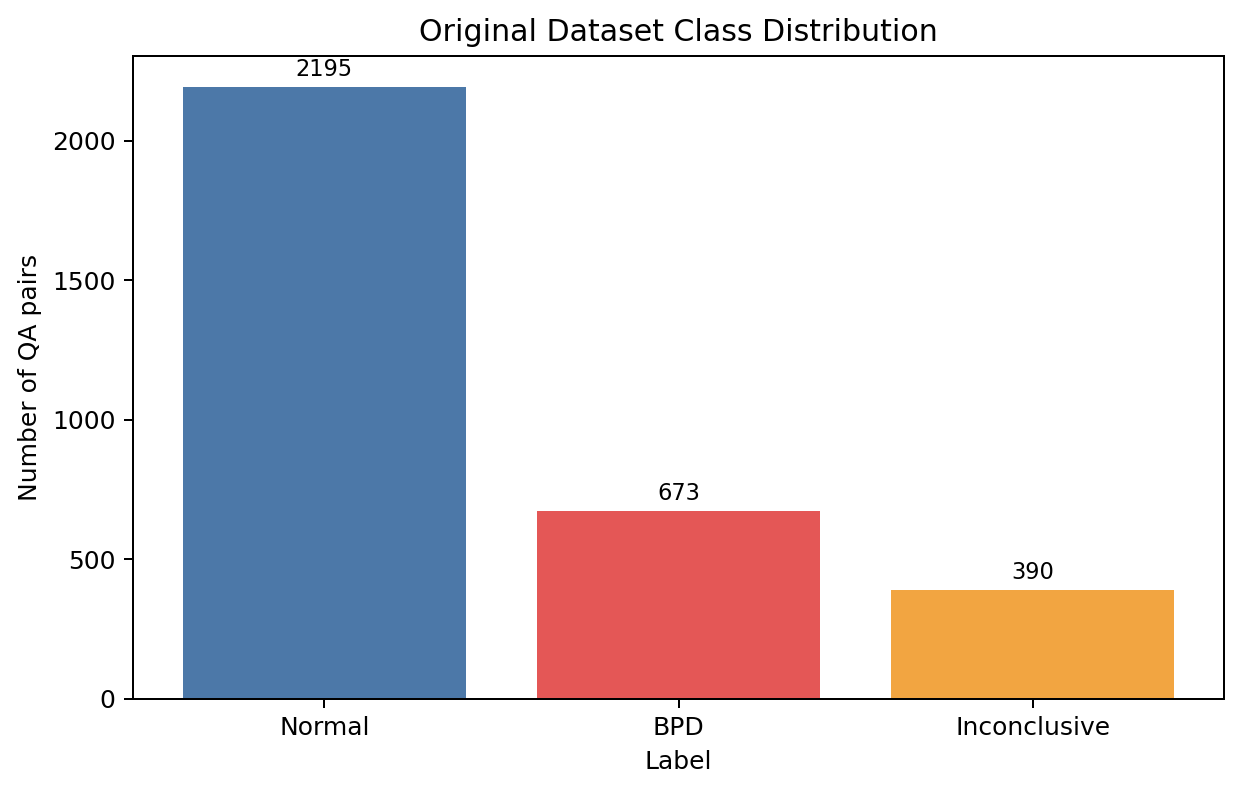
\includegraphics[width=0.75\linewidth]{generated/data_analysis/01_original_class_distribution.png}
\caption{Original class distribution of BPDQAC. The dataset is naturally imbalanced, with Normal responses forming the majority class.}
\label{fig:original_class_distribution}
\end{figure}

To address this issue during model development, augmentation was applied only to the training data. The original training subset contained 1,746 Normal responses, 538 BPD responses, and 308 Inconclusive responses. After augmentation, the training split was balanced to 1,746 instances per class, as illustrated in Figure~\ref{fig:augmentation_balance}. This balancing step is analytically relevant because it shows that the modelling pipeline was designed in response to a real dataset property rather than being imposed independently of the data.

\begin{figure}[H]
\centering
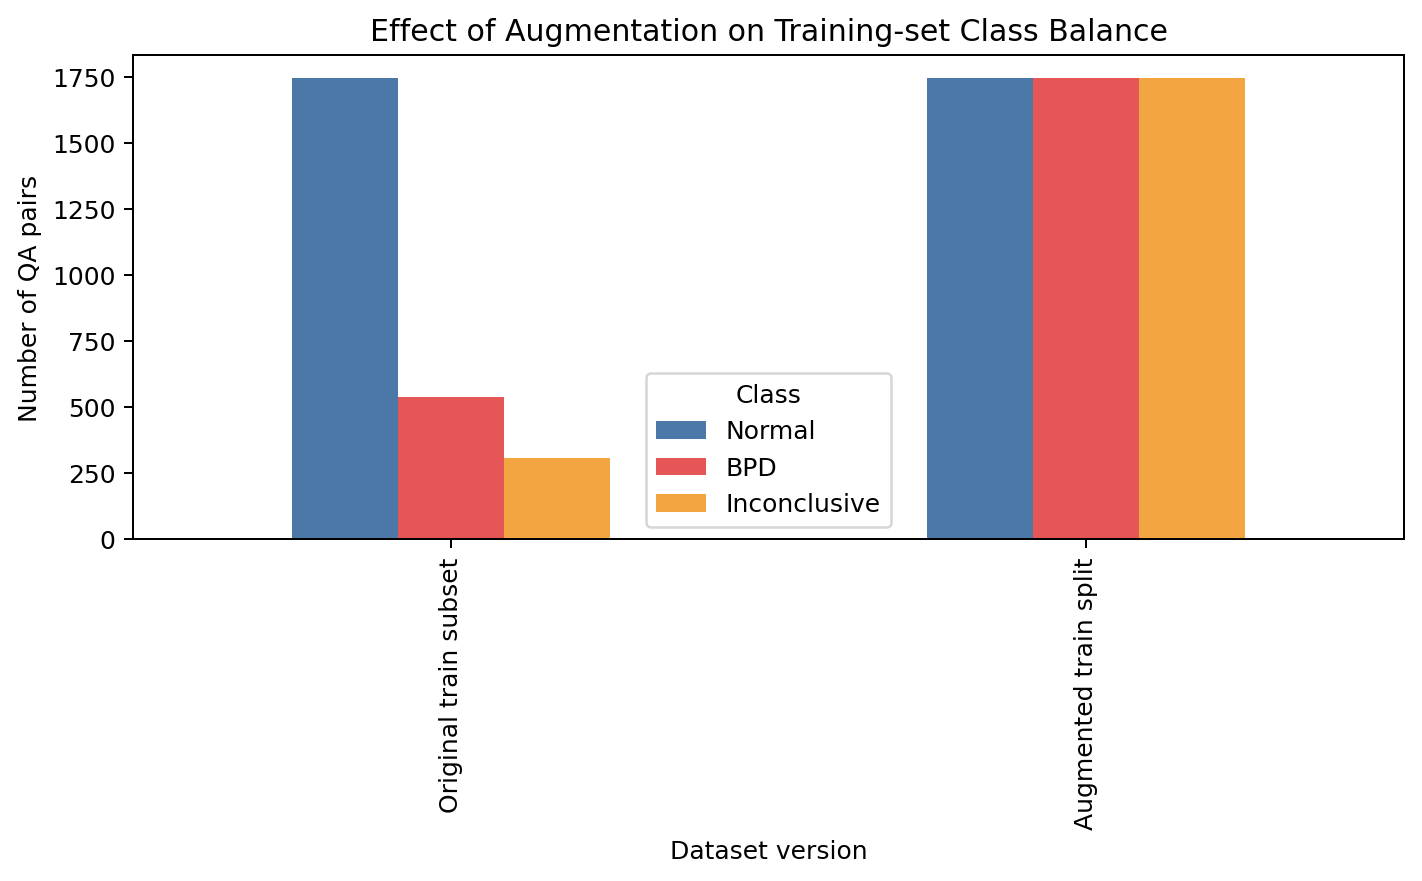
\includegraphics[width=0.82\linewidth]{generated/data_analysis/10_train_augmentation_comparison.png}
\caption{Effect of augmentation on the training-set class balance. The original training subset was strongly imbalanced, whereas the augmented training split was balanced across all three classes.}
\label{fig:augmentation_balance}
\end{figure}

\subsection{Question-Level Label Patterns}
The distribution of labels across questions is not uniform. Figure~\ref{fig:question_label_heatmap} shows the proportion of Normal, BPD, and Inconclusive labels for each of the nine diagnostic questions. Several questions appear more discriminative than others. Question 1, which targets abandonment-related experiences, yields the highest BPD proportion at approximately 0.33. Question 8, which targets anger and temper dysregulation, follows closely at 0.31. Questions 6 and 7, which address mood instability and chronic emptiness, also show comparatively elevated BPD proportions. In contrast, Question 5, which addresses self-harm and repeated suicide attempts, has the lowest BPD proportion at approximately 0.06 and the highest Normal share.

The figure also shows that Question 4, which targets impulsivity and self-damaging behaviors, produces the highest Inconclusive proportion at approximately 0.25. This suggests that some prompts may be more likely to elicit ambiguous or incomplete narratives. From an analysis perspective, this is an important property of the dataset because it indicates that the diagnostic prompts are not equally informative. Such heterogeneity can be useful for future work on prompt refinement, question weighting, or adaptive screening strategies.

\begin{figure}[H]
\centering
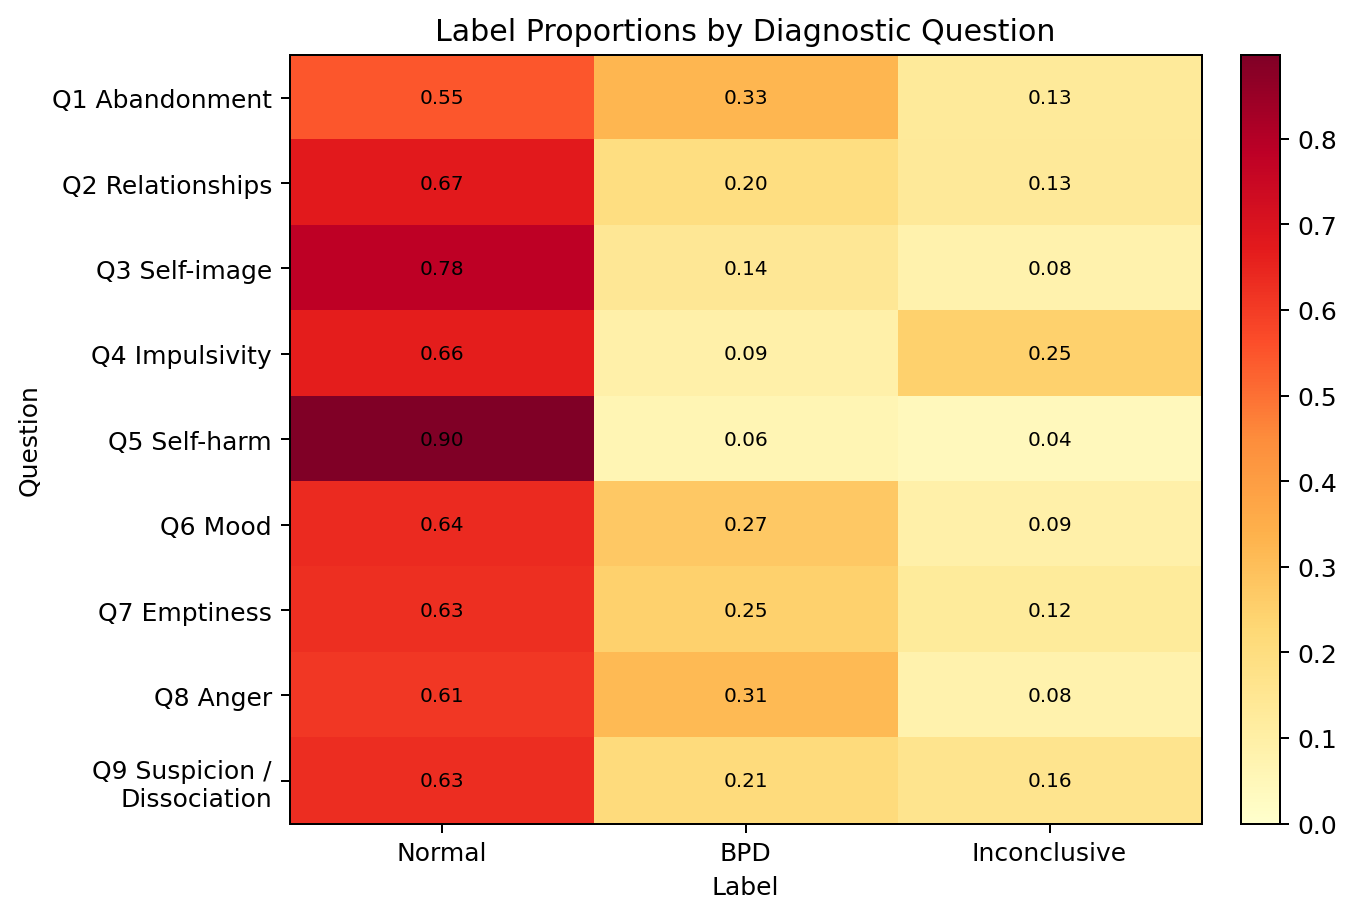
\includegraphics[width=0.82\linewidth]{generated/data_analysis/03_question_label_heatmap_refined.png}
\caption{Label proportions by diagnostic question. The figure shows that some questions are more strongly associated with BPD-labeled responses, while others yield more Normal or Inconclusive responses.}
\label{fig:question_label_heatmap}
\end{figure}

\subsection{Linguistic Characteristics of Responses}
The linguistic form of the responses also varies across classes. Figure~\ref{fig:answer_length_distributions} compares response length by label in terms of both word count and character count. BPD-labeled responses are the longest on average, with a mean length of 33.58 words, compared with 21.23 words for Normal responses and 18.24 words for Inconclusive responses. A similar pattern is observed in character count, where BPD responses are again the longest on average.

This difference suggests that BPD-indicative answers tend to be more elaborate and descriptive, whereas Inconclusive responses are often shorter and contain less decisive information. This is meaningful for publication because it shows that the labels are associated not only with class assignments but also with observable linguistic differences. In other words, the dataset contains measurable variation in textual behavior rather than only symbolic labels.

\begin{figure}[H]
\centering
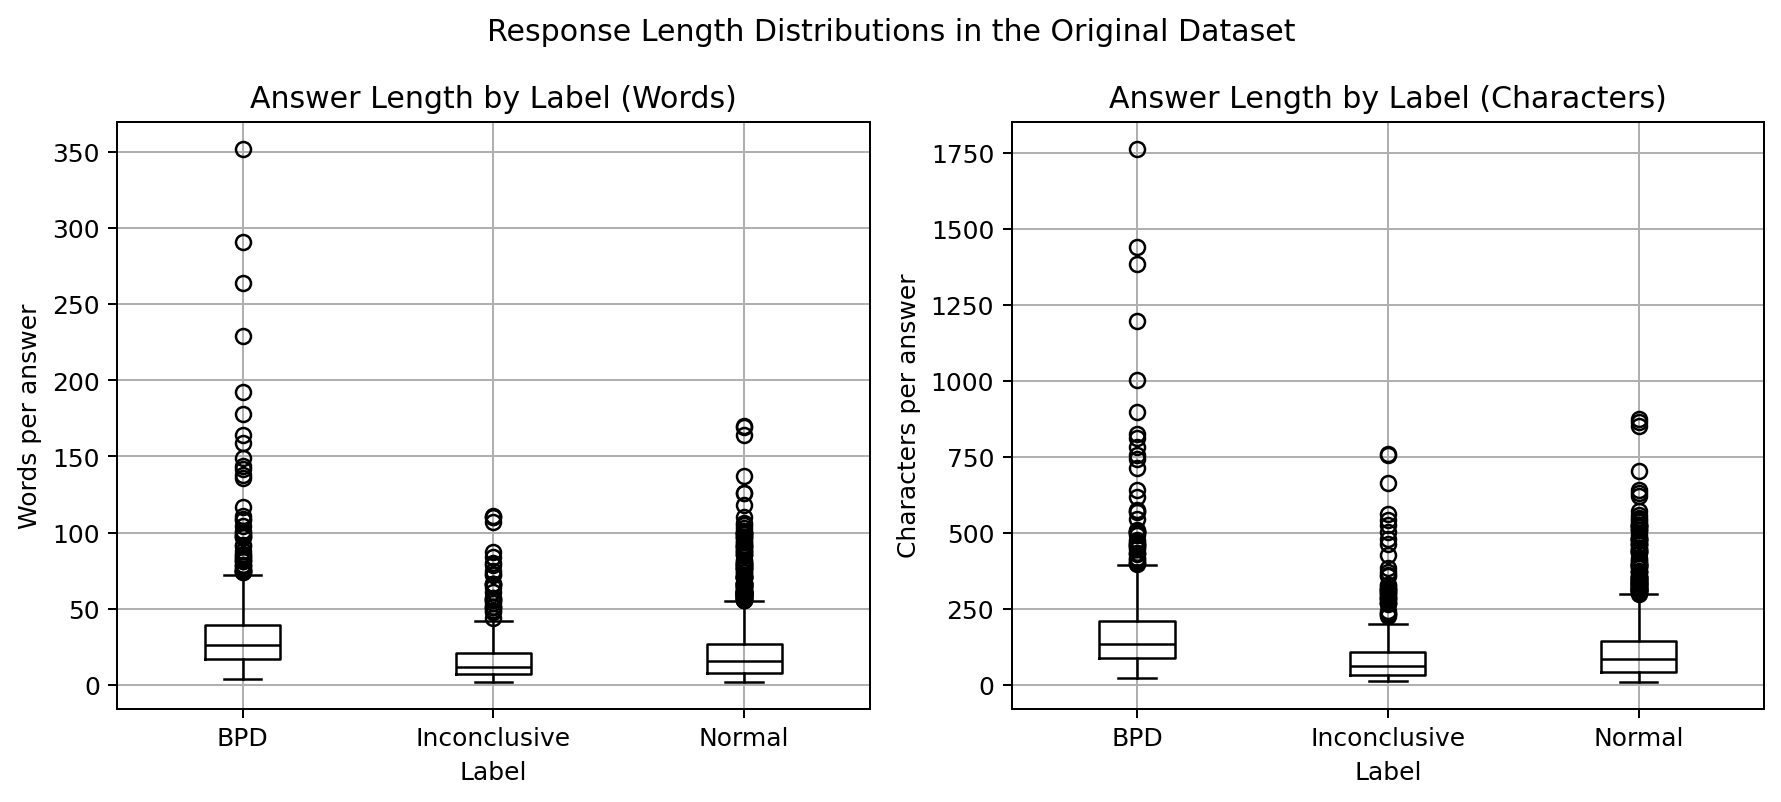
\includegraphics[width=\linewidth]{generated/data_analysis/04_answer_length_boxplots.png}
\caption{Response length distributions by label in the original dataset. BPD-labeled answers are generally longer than Normal and Inconclusive responses.}
\label{fig:answer_length_distributions}
\end{figure}

\subsection{Criteria B--F Response Patterns}
The five auxiliary Criteria B--F items were included to support structured screening at the participant level. Their behavior across labels is shown in Figure~\ref{fig:criteria_yes_rates}. Criteria B, C, and D display the clearest differences between classes. The BPD group has the highest yes-rates for Criterion B (0.511), Criterion C (0.560), and Criterion D (0.441), while the corresponding Normal proportions are 0.345, 0.394, and 0.303. These differences indicate that the supporting criteria contribute useful information beyond the open-ended Criterion A responses.

By contrast, Criteria E and F show very high yes-rates across all classes. In the original dataset, Criterion E is endorsed by 0.841 of the BPD group, 0.890 of the Inconclusive group, and 0.896 of the Normal group. Criterion F follows a similar pattern. This suggests that these two items may function more as broad exclusion conditions than as strong class separators in this population. This is a useful analytical finding because it highlights that not every DSM-aligned supporting criterion contributes equally to label differentiation in a screening dataset.

\begin{figure}[H]
\centering
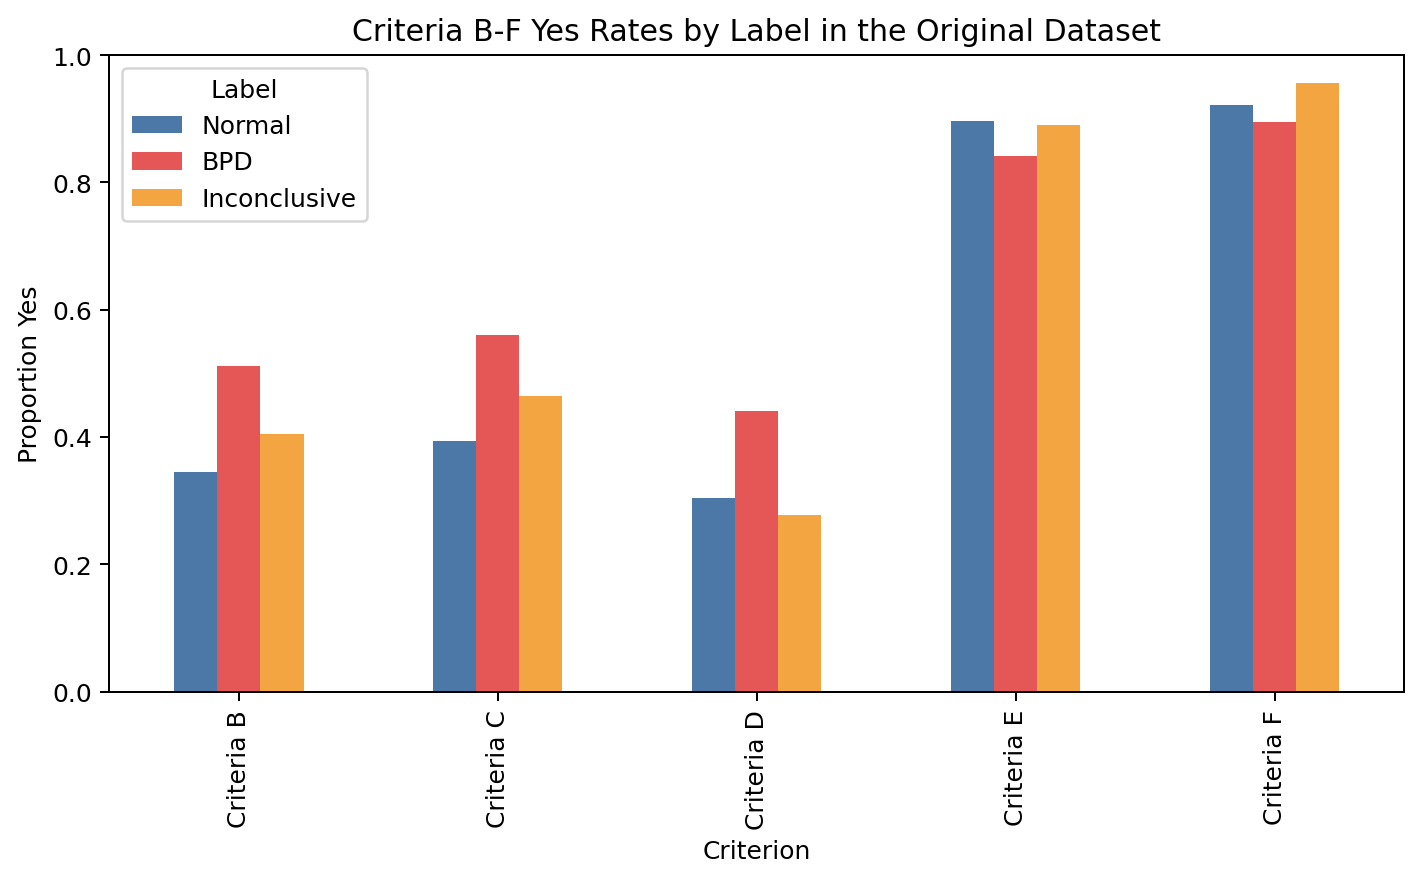
\includegraphics[width=0.85\linewidth]{generated/data_analysis/05_criteria_yes_rates.png}
\caption{Yes-rates for Criteria B--F across the three label groups. Criteria B, C, and D show greater separation across labels than Criteria E and F.}
\label{fig:criteria_yes_rates}
\end{figure}

\subsection{Participant-Level Screening Patterns}
Because BPDQAC supports participant-level aggregation, the dataset can also be examined through the proposed screening rule. Figure~\ref{fig:screening_rule_heatmap} shows participant counts according to two aggregated measures: the number of Criterion A responses labeled as BPD and the number of affirmative responses across Criteria B--F. The red dashed lines indicate the thresholds used in the screening rule: at least five BPD-labeled Criterion A responses and at least three affirmative Criteria B--F responses.

The distribution is concentrated in the lower-left and middle regions of the figure, indicating that most participants do not satisfy both thresholds simultaneously. Only 23 of the 362 participants satisfy the full rule, corresponding to approximately 6.4\% of the dataset. This is analytically important because it shows that the participant-level decision rule is selective rather than trivially permissive. The figure therefore helps connect the row-level classification structure of the dataset with its intended use in structured screening.

\begin{figure}[H]
\centering
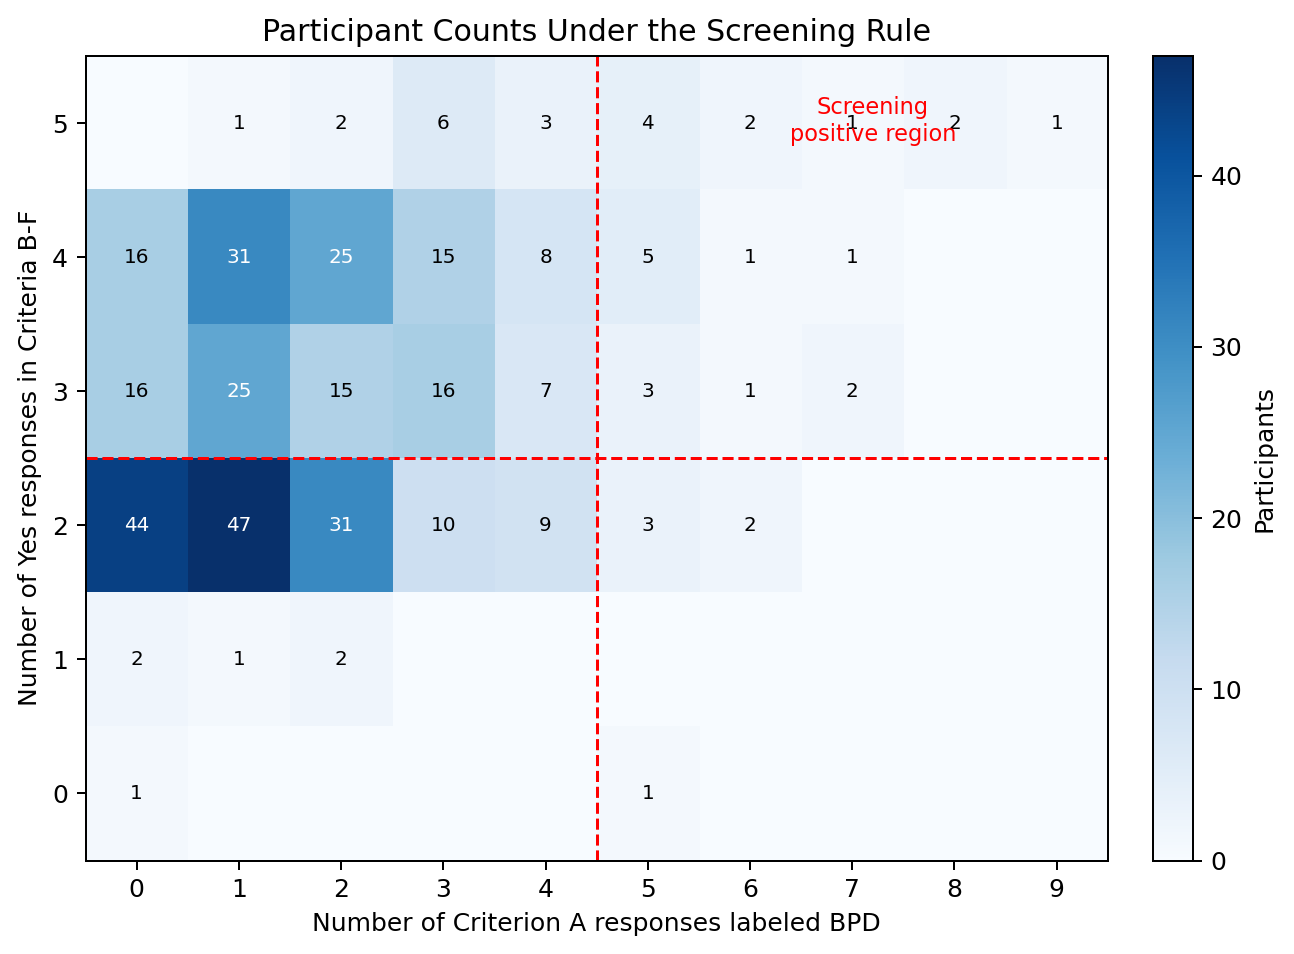
\includegraphics[width=0.82\linewidth]{generated/data_analysis/07_screening_rule_heatmap_refined.png}
\caption{Participant counts under the screening rule. The upper-right region beyond the red dashed thresholds corresponds to screening-positive participants.}
\label{fig:screening_rule_heatmap}
\end{figure}

\section{Technical Validation}\label{sec6}
This section documents the procedures and results used to assess the quality, reliability, and suitability of the released text dataset for supervised diagnostic modelling of borderline personality disorder. The validation focuses on (1) data integrity and representativeness, (2) annotation quality, (3) baseline predictive performance, and (4) robustness and fairness checks.


\subsection{Data Completeness}
Each of the nine open-ended questions was assigned a unique question\_id, and each participant was assigned a unique participant\_id. The dataset is organized systematically so that every participant contributes one response to each of the nine Criterion A questions. As a result, the dataset contains 362 records for each question\_id and 3,258 row-level question-answer entries in total.

The Criteria B--F responses are recorded for every participant and repeated across that participant's nine row-level entries. This arrangement makes it possible to analyze the data both at the response level and at the aggregated participant level. The dataset exhibits full data coverage, with no null or missing values in the released fields.

\subsection{Data Exclusion}

Responses containing clearly non-informative patterns were removed or normalized during preprocessing. These included uninterrupted character repetition, excessive punctuation, extended whitespace, emojis, keyboard-mashing, and incoherent text fragments without semantic value. Such patterns were treated as noise because they could distort annotation quality and reduce the reliability of downstream modelling. The exclusion criteria were therefore applied to preserve the interpretability and analytical quality of the dataset.

\subsection{Text Analysis}
The textual portion of BPDQAC consists of short to medium-length natural language responses produced under a structured questionnaire setting. This distinguishes the dataset from open-domain social media corpora, where topics, context, and speaker intent are often uncontrolled. Because the responses are elicited through clinically motivated prompts, the linguistic content is more directly tied to symptoms and diagnostic context. At the same time, the answers remain varied in wording, detail, and clarity, which preserves the natural language complexity necessary for realistic screening-oriented classification.

\subsection{Annotation Process}
To ensure diagnostic relevance and labeling consistency, annotation was carried out through a staged expert-guided process. Each question-answer pair received one of three labels: 0 for Normal, 1 for BPD, and 2 for Inconclusive. These labels reflect whether a response shows little to no sign of the target criterion, clear evidence consistent with the criterion, or insufficient information for a confident decision.

The initial half of the dataset was annotated independently by the three experts described above. Their labels were compiled to produce a verified seed set. A semi-supervised label propagation algorithm was then applied to assign provisional labels to the remaining half of the dataset. All generated labels were subsequently reviewed by the same experts, and disputed cases were discussed until agreement was reached. This process reduced annotation burden while maintaining expert control over the final released dataset.

The final annotation protocol combines three important properties: clinical grounding through expert review, consistency through label compilation and conflict resolution, and scalability through semi-supervised assistance. These properties support the use of BPDQAC as a supervised screening dataset while preserving a transparent link between the labels and the underlying diagnostic framework.

\section{Methodology}\label{sec3}
This section describes the modelling and evaluation workflow applied to BPDQAC after the dataset construction process described in Section~\ref{sec2}. Figure~\ref{fig:methodology_workflow} summarizes the complete workflow adopted in this work, including text processing, class balancing, model development, evaluation, explainability analysis, and deployment-oriented interface design.

\begin{figure}[H]
\centering
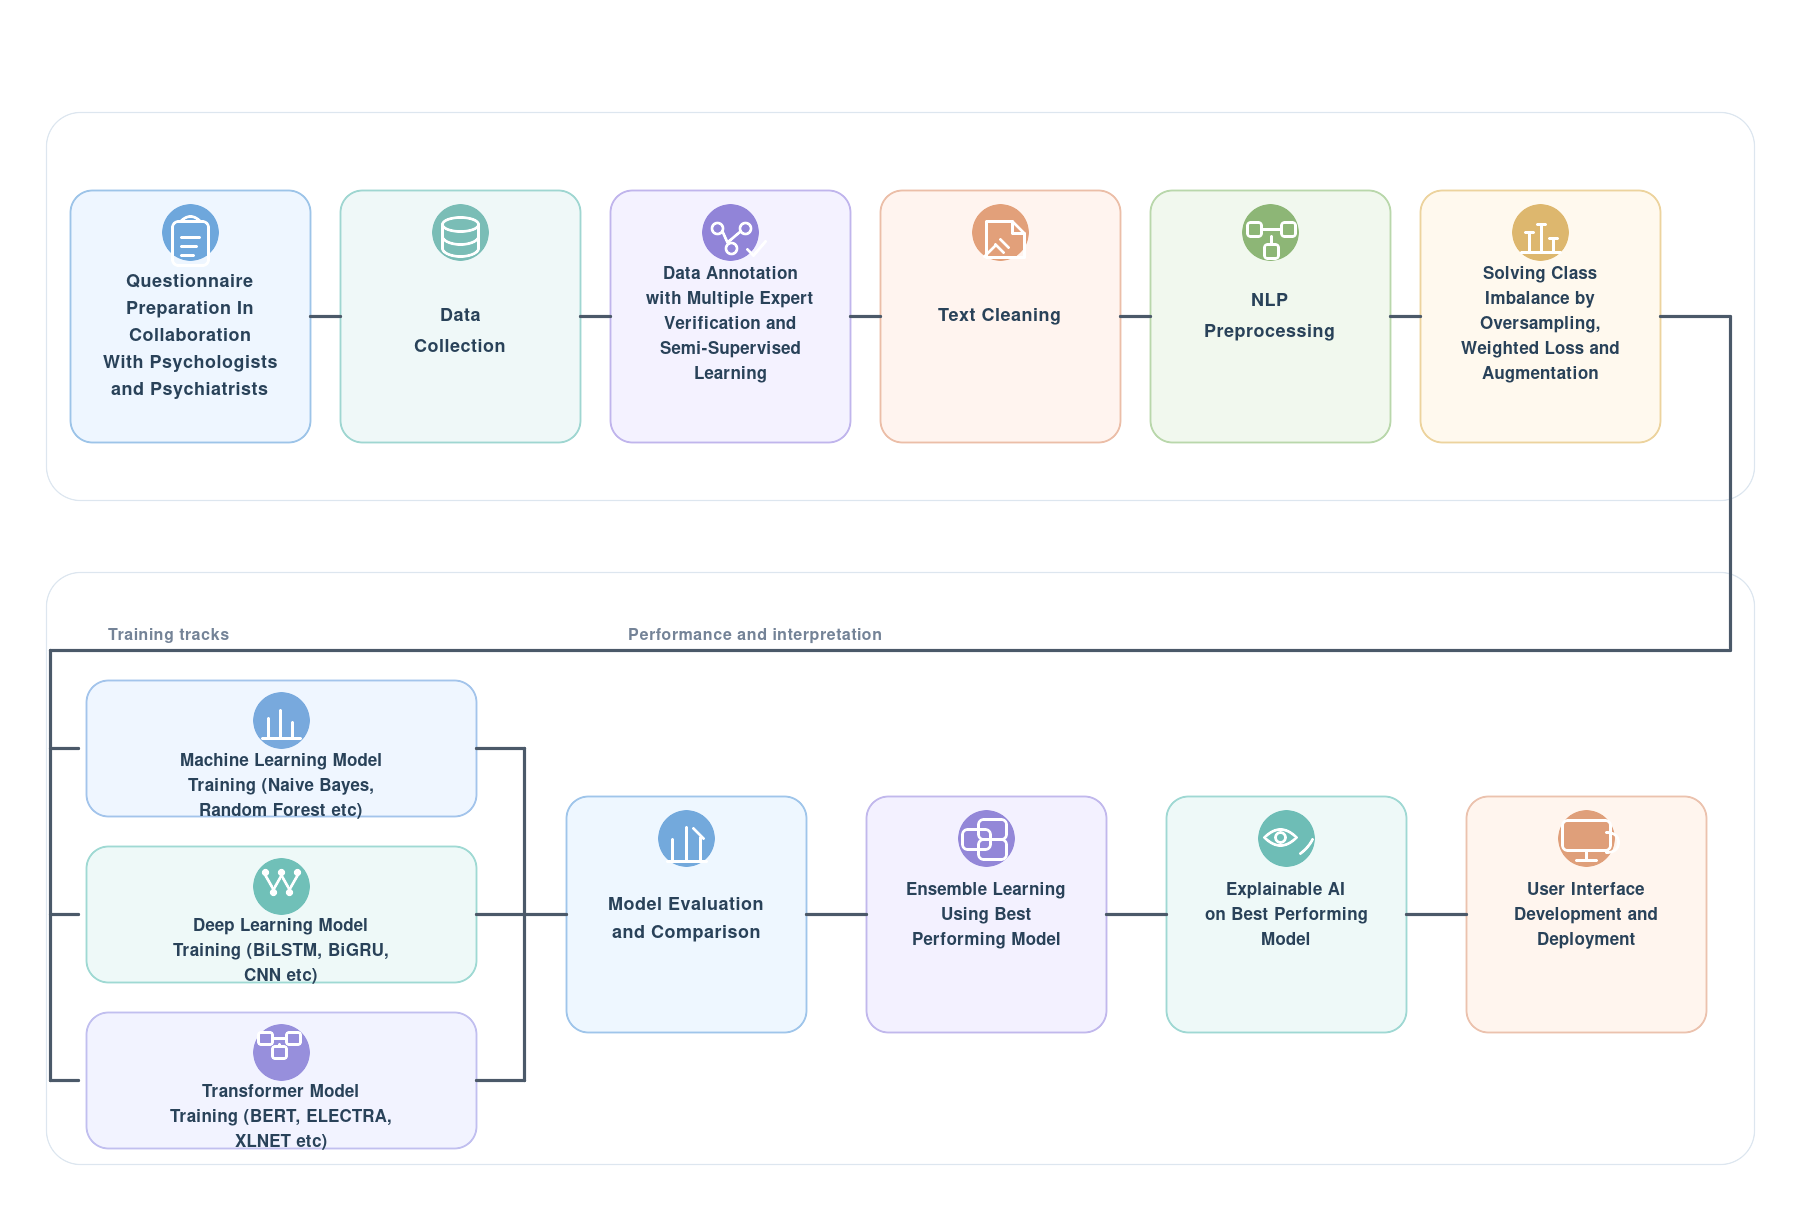
\includegraphics[width=\textwidth]{generated/figures/methodology_workflow_v4.png}
\caption{Overall methodological workflow of the study. The upper panel summarizes dataset construction and preparation, while the lower panel summarizes the modelling, evaluation, explainability, and deployment stages.}
\label{fig:methodology_workflow}
\end{figure}

The upper panel of Figure~\ref{fig:methodology_workflow} presents the stages used to construct BPDQAC, including DSM-5-guided questionnaire formulation, response collection, expert annotation, text cleaning, preprocessing, and class-imbalance handling. The lower panel presents the broader modelling pipeline considered during system development. Although the complete workflow accommodates traditional machine learning, deep learning, and transformer-based approaches, the finalized experiments reported in this paper focus on the transformer branch trained on the augmented dataset split, as this branch was retained as the primary experimental setting in the final notebook implementation.

\subsection{Model Training and Evaluation}
Each record in the modelling phase was treated as a three-class question-answer classification instance, where the target labels were \textit{Normal}, \textit{BPD}, and \textit{Inconclusive}. The final notebook implementation uses the augmented dataset split directly, with 5,238 training samples, 333 validation samples, and 333 test samples. This experimental setting reflects the final augmented-data workflow preserved in the notebook, whereas raw-data baselines, weighted-loss variants, and ensemble sections were retained only as exploratory scaffolding and were not used as the main reported training pipeline.

\subsubsection{Text Preprocessing and Input Representation}
Before tokenization, both the \texttt{question} and \texttt{answer} fields were normalized to reduce informal variation in participant responses. The preprocessing pipeline converted text to lowercase, removed unnecessary special characters while preserving basic punctuation, expanded contractions, and replaced common slang and domain abbreviations through a manually defined normalization dictionary. This step was applied consistently to the training, validation, and test splits.

For encoder-based transformers, each sample was represented as a paired input consisting of the diagnostic question and the corresponding participant response. Tokenization was performed jointly on the two text fields with truncation enabled, and dynamic padding was handled at batch time through a padding-aware data collator. In the T5 setting, each sample was reformulated as a prompted sequence of the form \texttt{trinary classification: <question> </s> <answer>}, allowing the model to process the task in a text-to-text style while still producing a three-class decision through a sequence-classification head.

\subsubsection{Evaluated Models and Fine-Tuning Configuration}
Eight transformer models were evaluated in the final experimental setup: ELECTRA-base, BERT-base, DistilBERT-base, RoBERTa-base, XLNet-base, DeBERTa-v3-base, ModernBERT-base, and T5-small. All models were fine-tuned using the Hugging Face \texttt{Trainer} API for a maximum of 15 epochs. Evaluation, logging, and checkpoint saving were performed at the end of each epoch. The best checkpoint for each model was selected using the lowest validation loss, and early stopping with a patience of two epochs was used to reduce unnecessary training once validation performance stopped improving.

Mixed-precision training was enabled when supported by the available hardware, and the notebook included a single-GPU stability mode for models that were more sensitive to runtime configuration. The principal training parameters are summarized in Table~\ref{tab:model_hyperparameters}. Since most settings were intentionally harmonized across models, the table highlights both the shared configuration and the few model-specific adjustments required for stable fine-tuning.

\begin{table}[H]
\centering
\caption{Training configuration of the evaluated transformer models.}
\label{tab:model_hyperparameters}
\scriptsize
\renewcommand{\arraystretch}{1.18}
\resizebox{\textwidth}{!}{%
\begin{tabular}{lcccccccc}
\hline
Parameter & ELECTRA & BERT & DistilBERT & RoBERTa & XLNet & DeBERTa & ModernBERT & T5 \\
\hline
Train batch size & 16 & 16 & 16 & 16 & 4 & 8 & 8 & 2 \\
Eval batch size & 16 & 16 & 16 & 16 & 2 & 8 & 8 & 2 \\
Gradient accumulation & 1 & 1 & 1 & 1 & 4 & 2 & 2 & 8 \\
Effective batch size & 16 & 16 & 16 & 16 & 16 & 16 & 16 & 16 \\
Epochs & 15 & 15 & 15 & 15 & 15 & 15 & 15 & 15 \\
Learning rate & $5\times10^{-6}$ & $5\times10^{-6}$ & $5\times10^{-6}$ & $5\times10^{-6}$ & $5\times10^{-6}$ & $2\times10^{-5}$ & $2\times10^{-5}$ & $5\times10^{-5}$ \\
Weight decay & 0.10 & 0.10 & 0.10 & 0.10 & 0.10 & 0.01 & 0.01 & 0.01 \\
Warmup ratio & 0.20 & 0.20 & 0.20 & 0.20 & 0.20 & 0.10 & 0.10 & 0.20 \\
LR scheduler & Linear & Linear & Linear & Linear & Linear & Linear & Linear & Linear \\
Evaluation strategy & Epoch & Epoch & Epoch & Epoch & Epoch & Epoch & Epoch & Epoch \\
Save strategy & Epoch & Epoch & Epoch & Epoch & Epoch & Epoch & Epoch & Epoch \\
Best-model criterion & Eval.\ loss & Eval.\ loss & Eval.\ loss & Eval.\ loss & Eval.\ loss & Eval.\ loss & Eval.\ loss & Eval.\ loss \\
Early stopping patience & 2 & 2 & 2 & 2 & 2 & 2 & 2 & 2 \\
Extra & -- & -- & -- & -- & \shortstack[c]{Left padding;\\pad token set;\\eval accumulation = 8} & \shortstack[c]{Stability retry\\after earlier\\class collapse} & -- & \shortstack[c]{Prompted input: \texttt{trinary classification:}\\\texttt{<question> </s> <answer>}} \\
\hline
\end{tabular}}
\end{table}

\subsubsection{Evaluation Protocol}
Model performance was assessed on the held-out augmented test split using accuracy, weighted precision, weighted recall, and weighted F1-score. Weighted averaging was selected because the original dataset is imbalanced, and the evaluation needed to reflect overall performance without ignoring the contribution of minority classes. In addition to aggregate metrics, class-wise classification reports were generated for the \textit{Normal}, \textit{BPD}, and \textit{Inconclusive} classes in order to examine how well each model handled the clinically important minority labels.

The final comparison among models was based primarily on weighted F1-score, with accuracy, precision, and recall used as supporting measures. During training, model selection was driven by validation loss rather than test performance, which helps separate model selection from final evaluation. This protocol keeps the experiments aligned with standard supervised learning practice while remaining suitable for a clinically motivated text classification dataset of moderate size.

\section{Results}\label{sec7}

\subsection{Encoder Model Performance}
To examine whether BPDQAC supports supervised diagnostic modelling beyond surface-level lexical matching, a family of encoder-based transformer classifiers was evaluated on the three-class question-answer classification task. The encoder experiments used an augmented training split of 5,238 samples together with 333 validation samples and 333 held-out test samples. Model ranking was based primarily on weighted F1-score, while accuracy, precision, and recall were reported as complementary measures under the observed class imbalance in the test set (225 Normal, 67 BPD, and 41 Inconclusive responses).

Table~\ref{tab:encoder_model_results} summarizes the encoder results. XLNet achieved the strongest overall performance, with a test accuracy of 0.862 and a weighted F1-score of 0.862. ELECTRA followed closely, reaching 0.856 accuracy and 0.854 weighted F1-score, which indicates that the proposed dataset supports stable learning across more than one encoder architecture. ModernBERT and RoBERTa formed a second tier, both exceeding 0.82 weighted F1-score, while DistilBERT and BERT remained competitive but produced a larger drop in overall discrimination. In contrast, DeBERTa underperformed substantially, obtaining 0.676 accuracy and a weighted F1-score of 0.545, which suggests that this configuration failed to adapt reliably to the dataset despite the same task formulation.

\begin{table}[H]
\centering
\scriptsize
\captionsetup{width=0.72\linewidth, justification=centering, singlelinecheck=false}
\caption{Test-set performance of encoder-based transformer models on BPDQAC.}
\label{tab:encoder_model_results}
\setlength{\tabcolsep}{3pt}
\renewcommand{\arraystretch}{0.9}
\begin{tabular}{@{}lcccc@{}}
\hline
Model & Accuracy & Weighted F1 & Precision & Recall \\
\hline
XLNet & 0.862 & 0.862 & 0.867 & 0.862 \\
ELECTRA & 0.856 & 0.854 & 0.855 & 0.856 \\
ModernBERT & 0.832 & 0.824 & 0.826 & 0.832 \\
RoBERTa & 0.820 & 0.822 & 0.832 & 0.820 \\
DistilBERT & 0.799 & 0.806 & 0.824 & 0.799 \\
BERT & 0.790 & 0.795 & 0.803 & 0.790 \\
DeBERTa & 0.676 & 0.545 & 0.457 & 0.676 \\
\hline
\end{tabular}
\end{table}

The relative separation between encoder models is also visible in Figure~\ref{fig:encoder_metric_comparison}, where XLNet and ELECTRA maintain the most balanced profile across all four evaluation metrics. ModernBERT and RoBERTa remain strong alternatives, but their weighted F1-scores reveal a modest decline in class-sensitive performance compared with the two leading models. DeBERTa is the only encoder for which the metric profile clearly breaks down, with precision dropping sharply because the model collapsed toward majority-class predictions.

\begin{figure}[H]
\centering
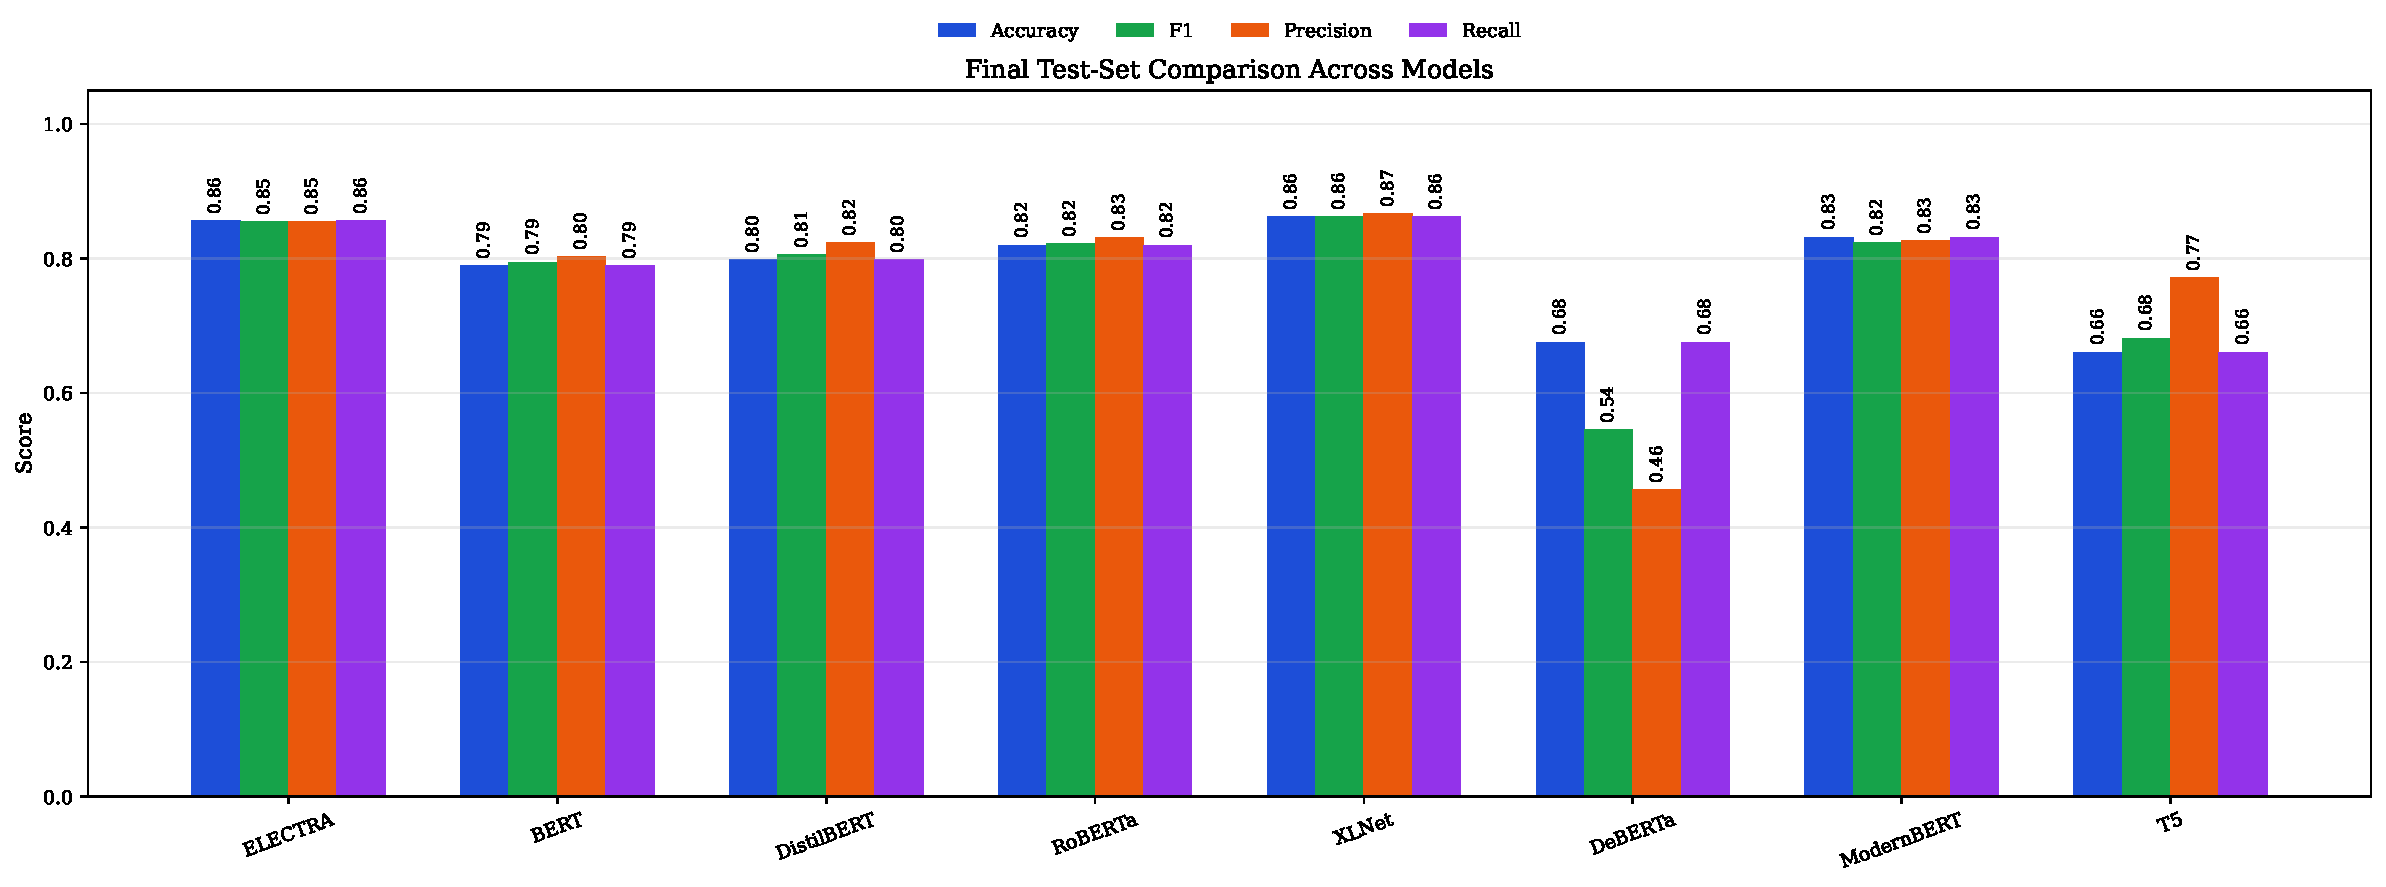
\includegraphics[width=\textwidth]{Figures/final_test_metric_comparison.pdf}
\caption{Final test-set comparison across the evaluated models. The present subsection focuses on the encoder-based models shown in the figure.}
\label{fig:encoder_metric_comparison}
\end{figure}

The optimization behaviour of the encoder models is further illustrated by the loss curves in Figure~\ref{fig:encoder_loss_curves}. XLNet, ELECTRA, RoBERTa, and ModernBERT show a consistent decline in training loss while maintaining comparatively lower validation loss than the weaker models, which supports their stronger final test performance. DistilBERT and BERT also exhibit stable optimization, but their validation losses plateau at a less favorable level, which is consistent with their middle-tier ranking in Table~\ref{tab:encoder_model_results}. DeBERTa displays the least desirable pattern: the training loss remains high and the validation loss trends upward, indicating that the model failed to learn a robust decision boundary for this dataset.

\begin{figure}[H]
\centering
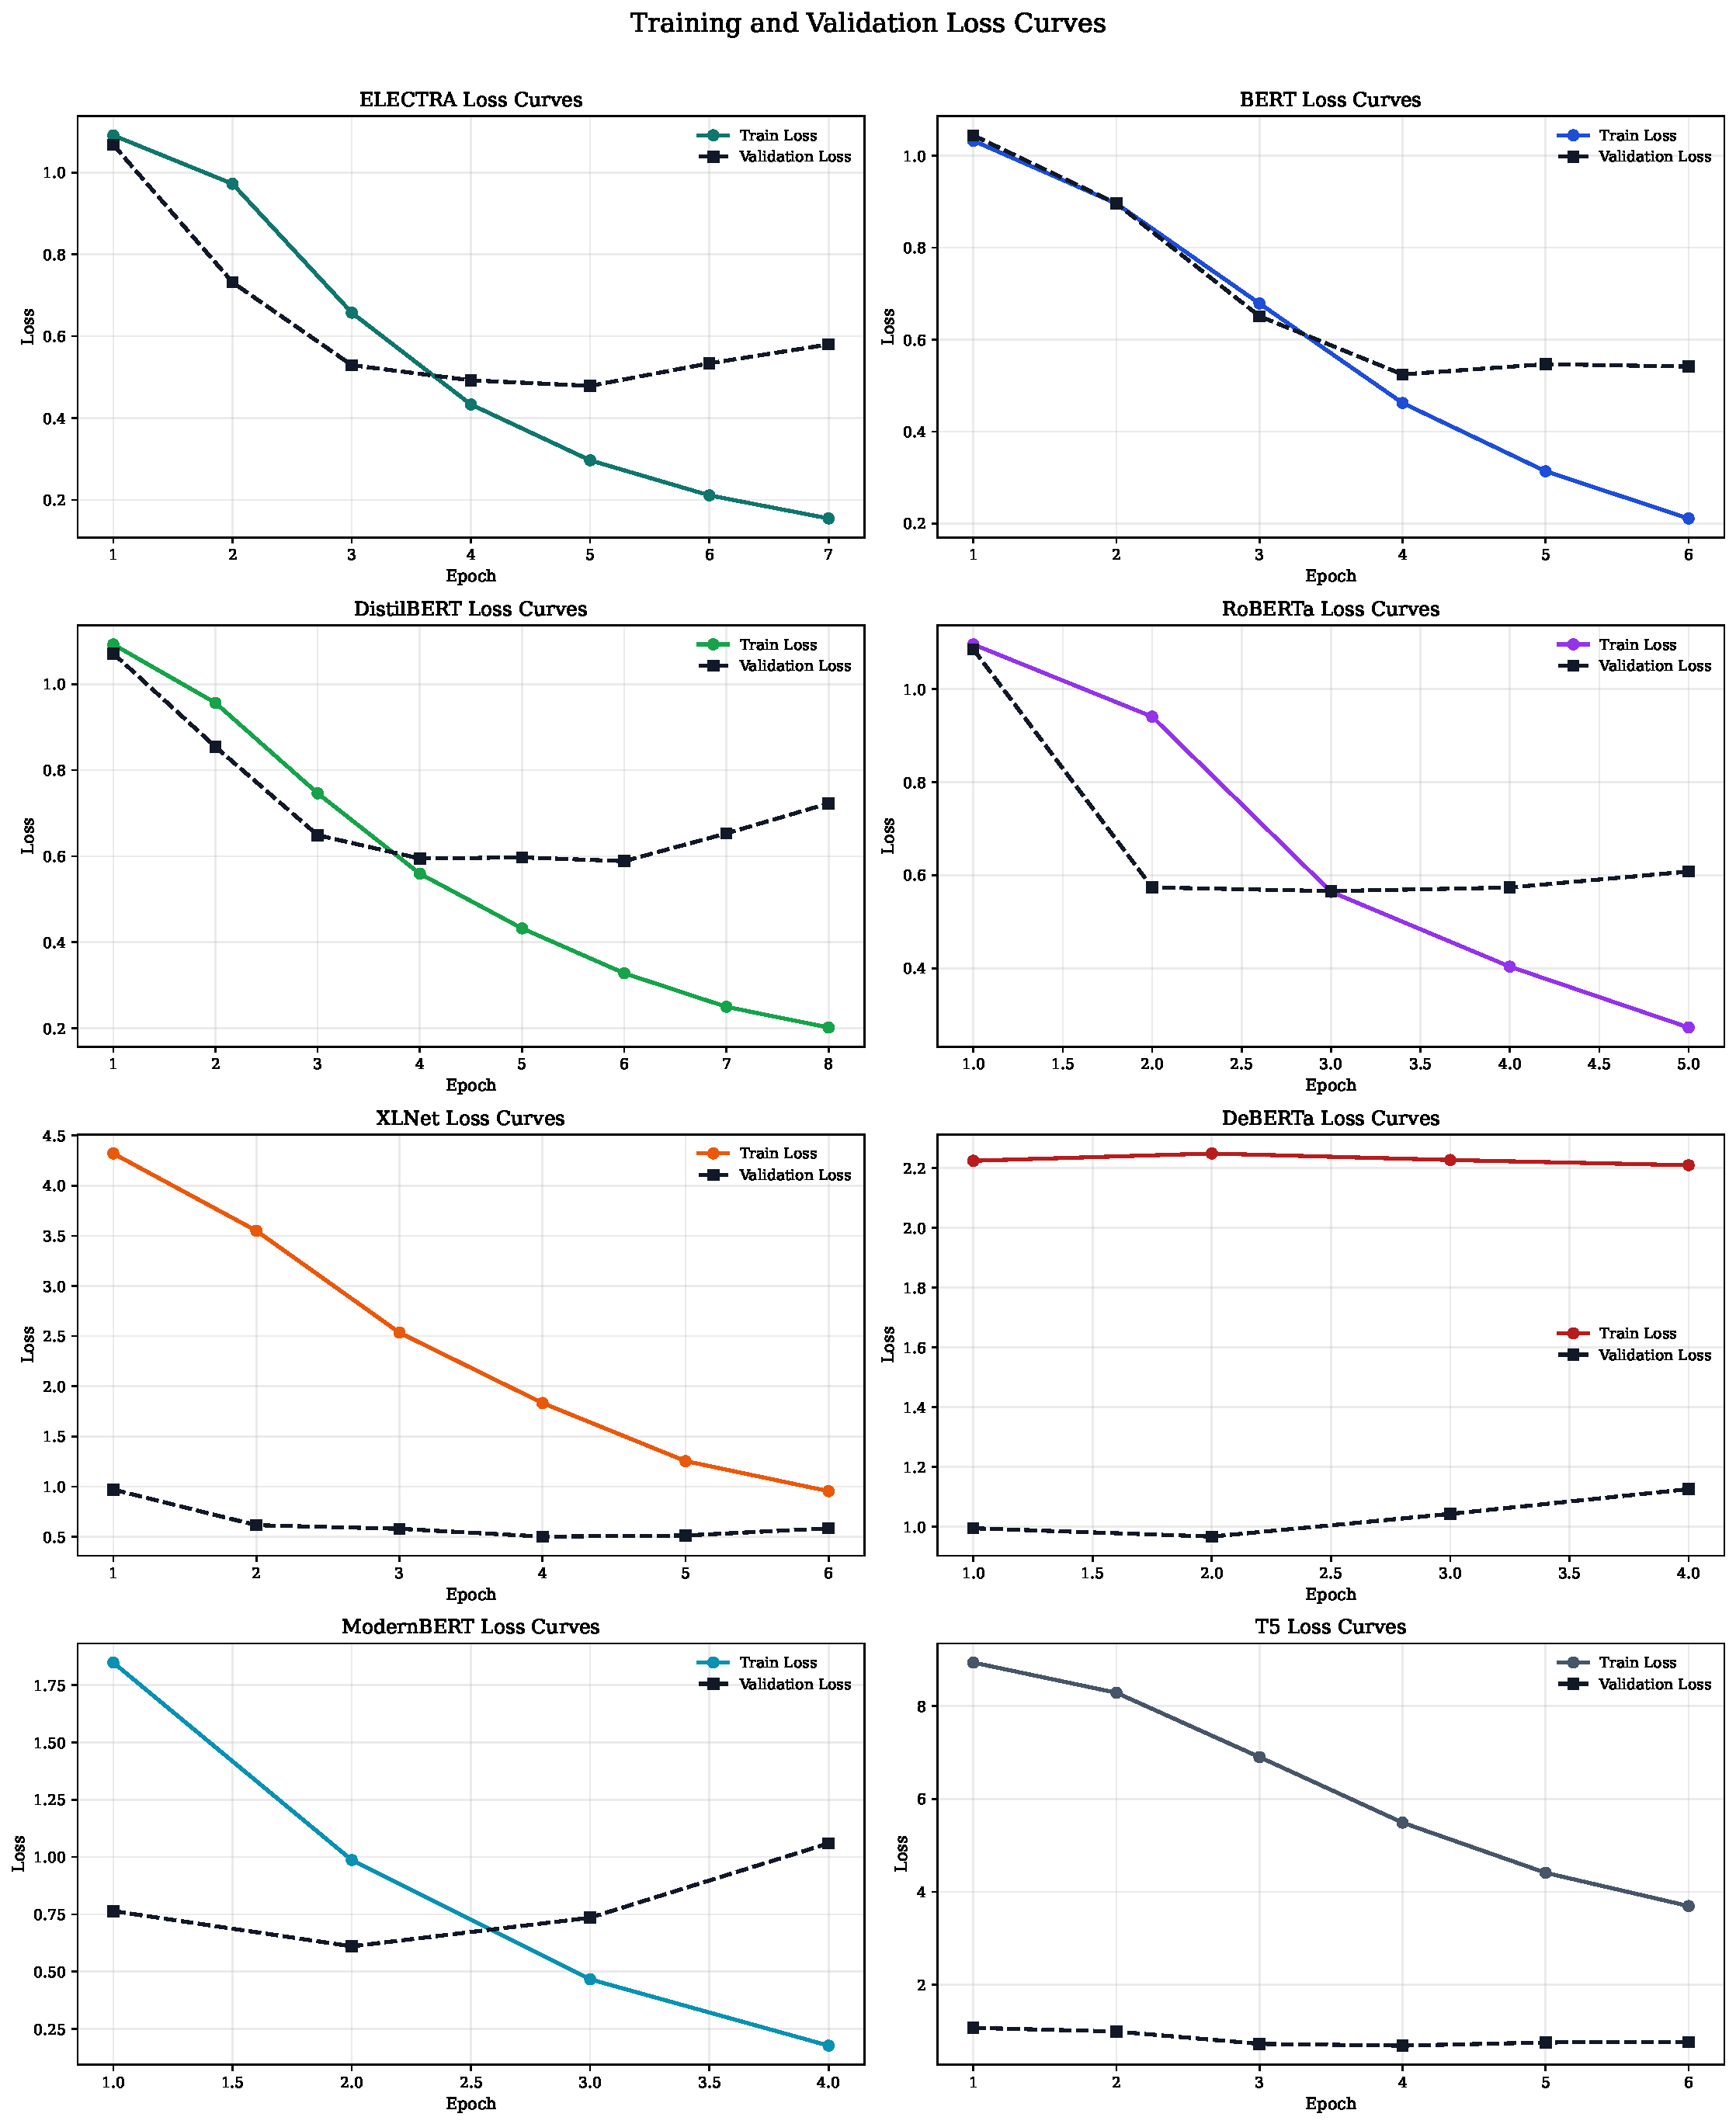
\includegraphics[width=\textwidth]{Figures/all_models_loss_curves.pdf}
\caption{Training and validation loss curves over epochs. The interpretation in this subsection focuses on the encoder-based models.}
\label{fig:encoder_loss_curves}
\end{figure}

The validation weighted F1-score trajectories in Figure~\ref{fig:encoder_validation_curves} provide additional evidence for the observed ranking. XLNet, ELECTRA, ModernBERT, and RoBERTa converged rapidly and then remained comparatively stable over subsequent epochs, indicating that diagnostically relevant patterns in the question-answer pairs can be learned consistently by several encoder families. DistilBERT and BERT improved more gradually but still converged toward usable decision boundaries. DeBERTa, however, exhibited a late-stage collapse in validation weighted F1-score, which is consistent with its weak generalization on the held-out test set.

\begin{figure}[H]
\centering
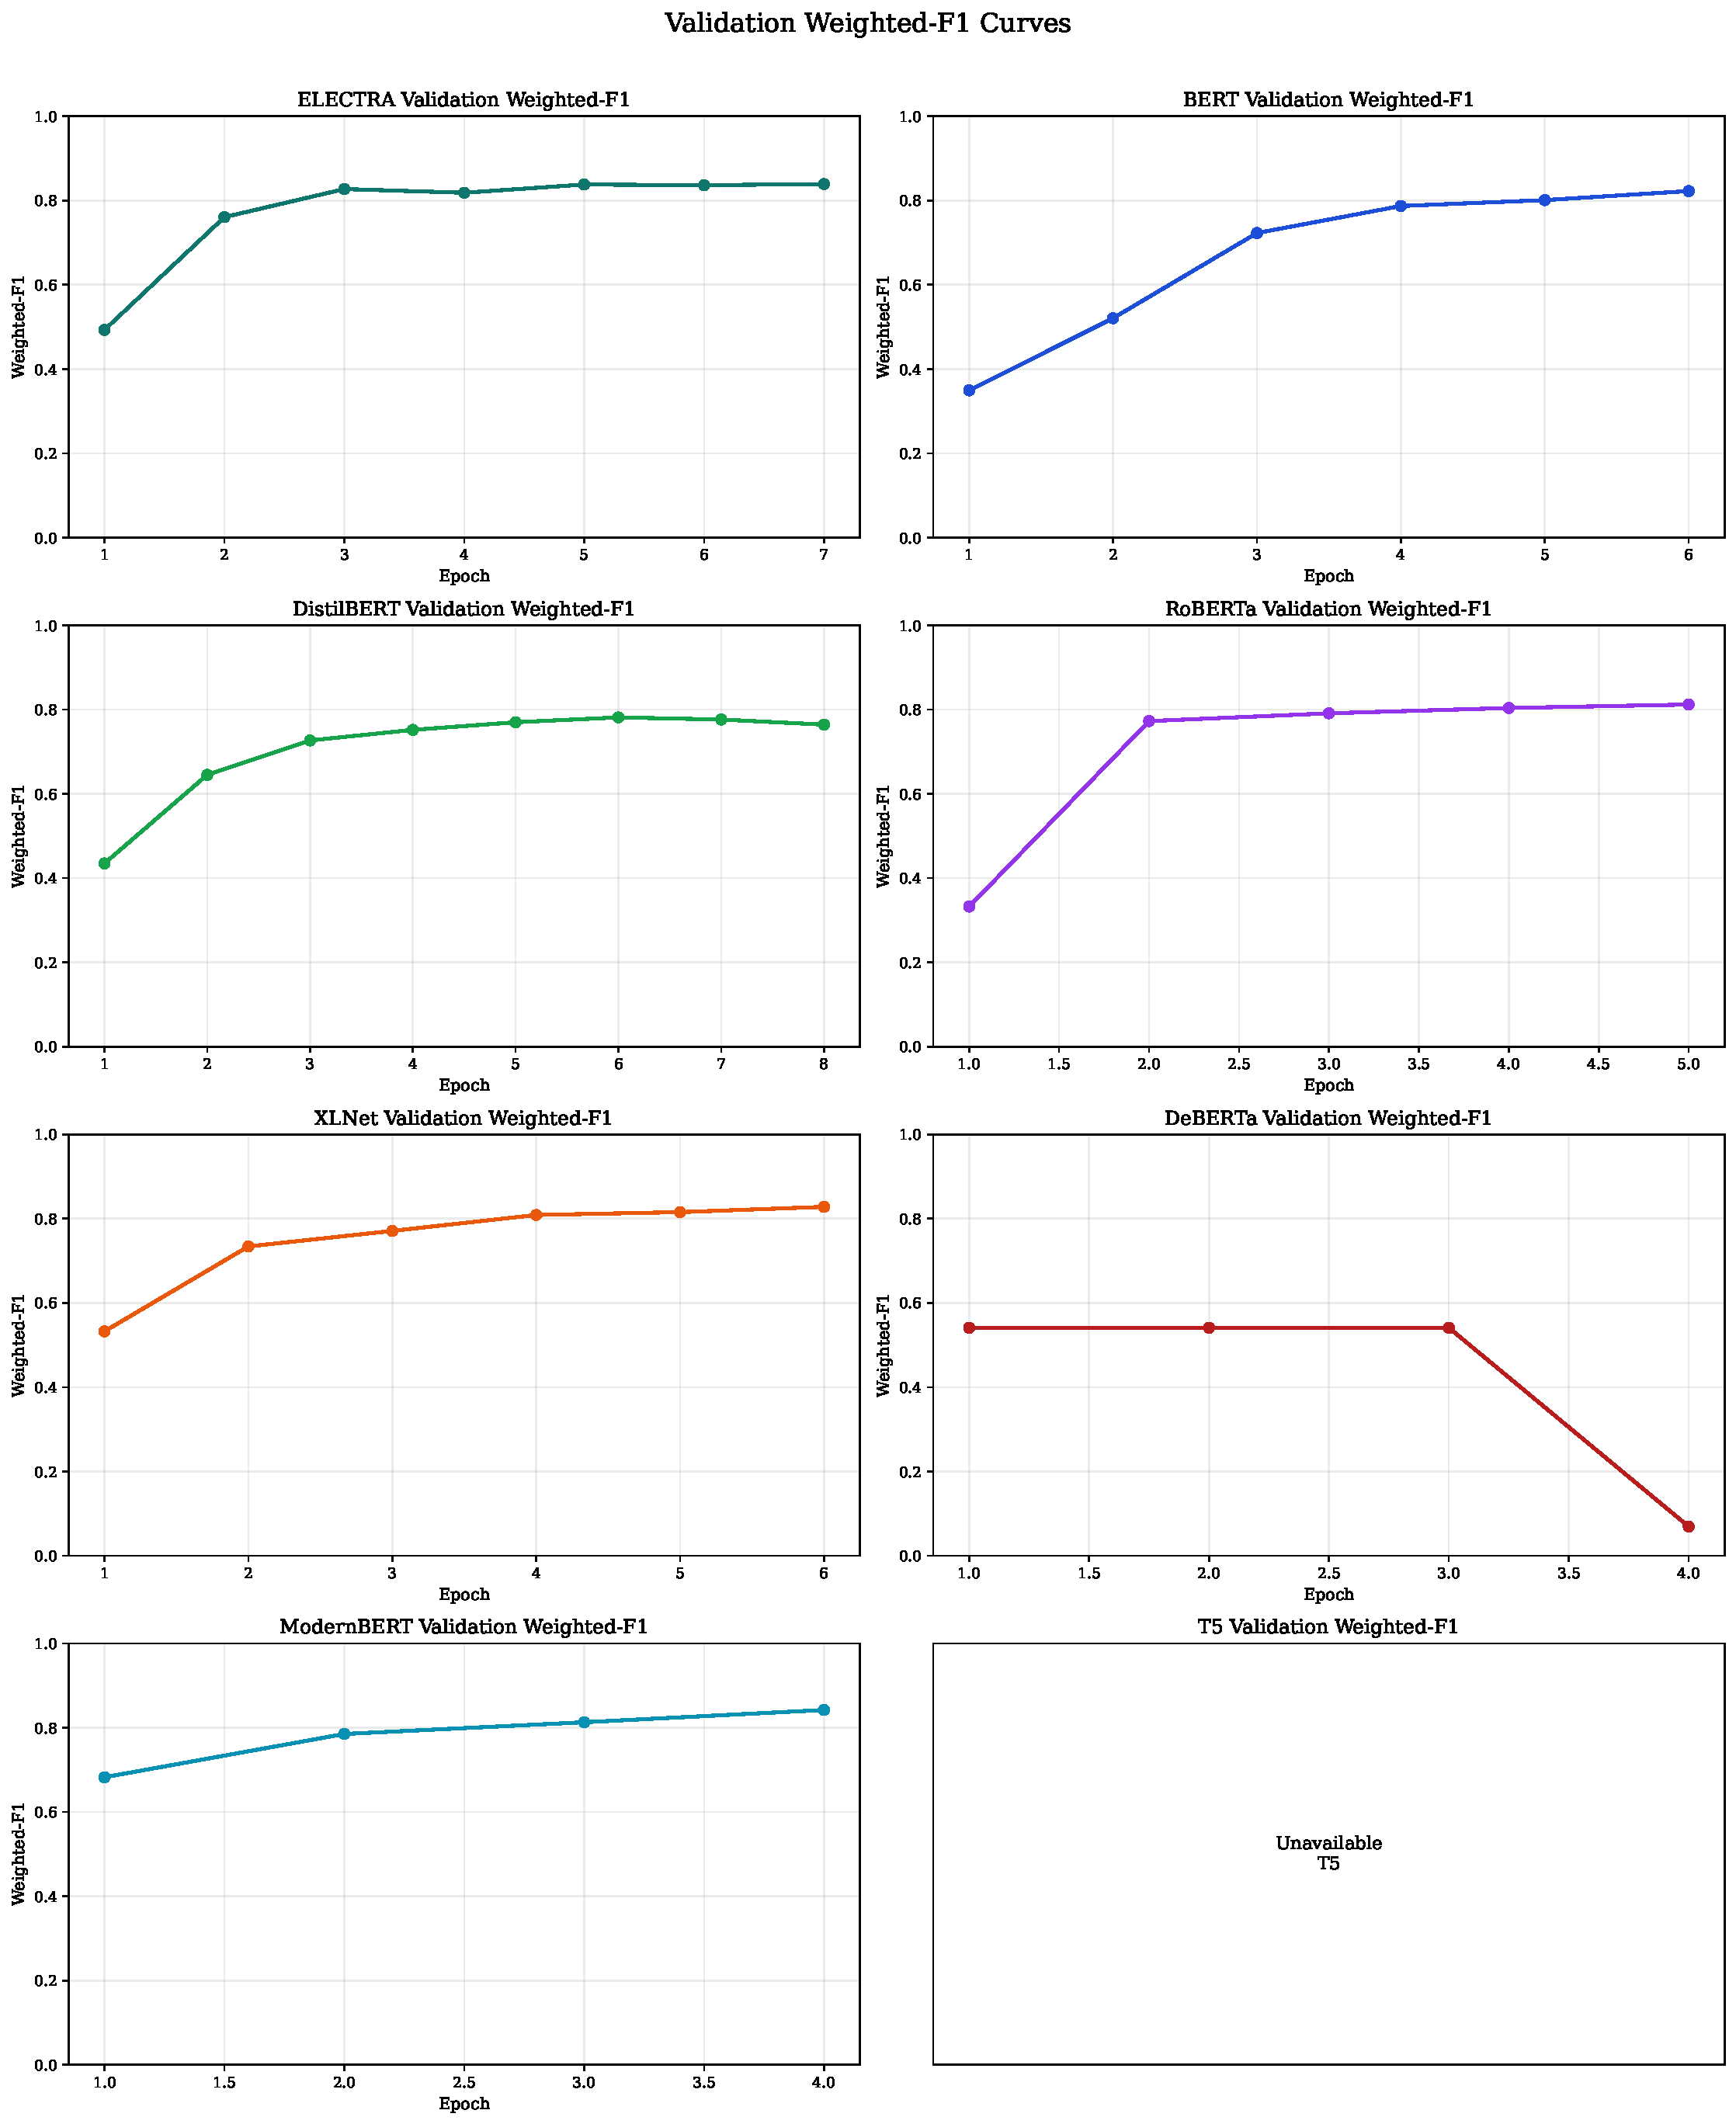
\includegraphics[width=\textwidth]{Figures/all_models_validation_weighted_f1.pdf}
\caption{Validation weighted F1-score curves over training epochs. Only the encoder-based models are interpreted in this subsection.}
\label{fig:encoder_validation_curves}
\end{figure}

The confusion matrices in Figure~\ref{fig:encoder_confusion_matrices} clarify how the encoder models behave at the class level. Across nearly all models, the Normal class was recognized most reliably, which is expected because it is the largest class in the evaluation split. More importantly, the strongest encoders retained meaningful sensitivity to BPD responses: XLNet correctly identified 56 of 67 BPD samples, ELECTRA identified 53, RoBERTa identified 55, and DistilBERT identified 54. This indicates that the dataset contains learnable disorder-related linguistic cues rather than only supporting majority-class recognition. The Inconclusive class remained the most challenging category for most encoders, reflecting the fact that ambiguous or weakly informative responses lie closer to the boundary between clinically indicative and non-indicative language.

\begin{figure}[H]
\centering
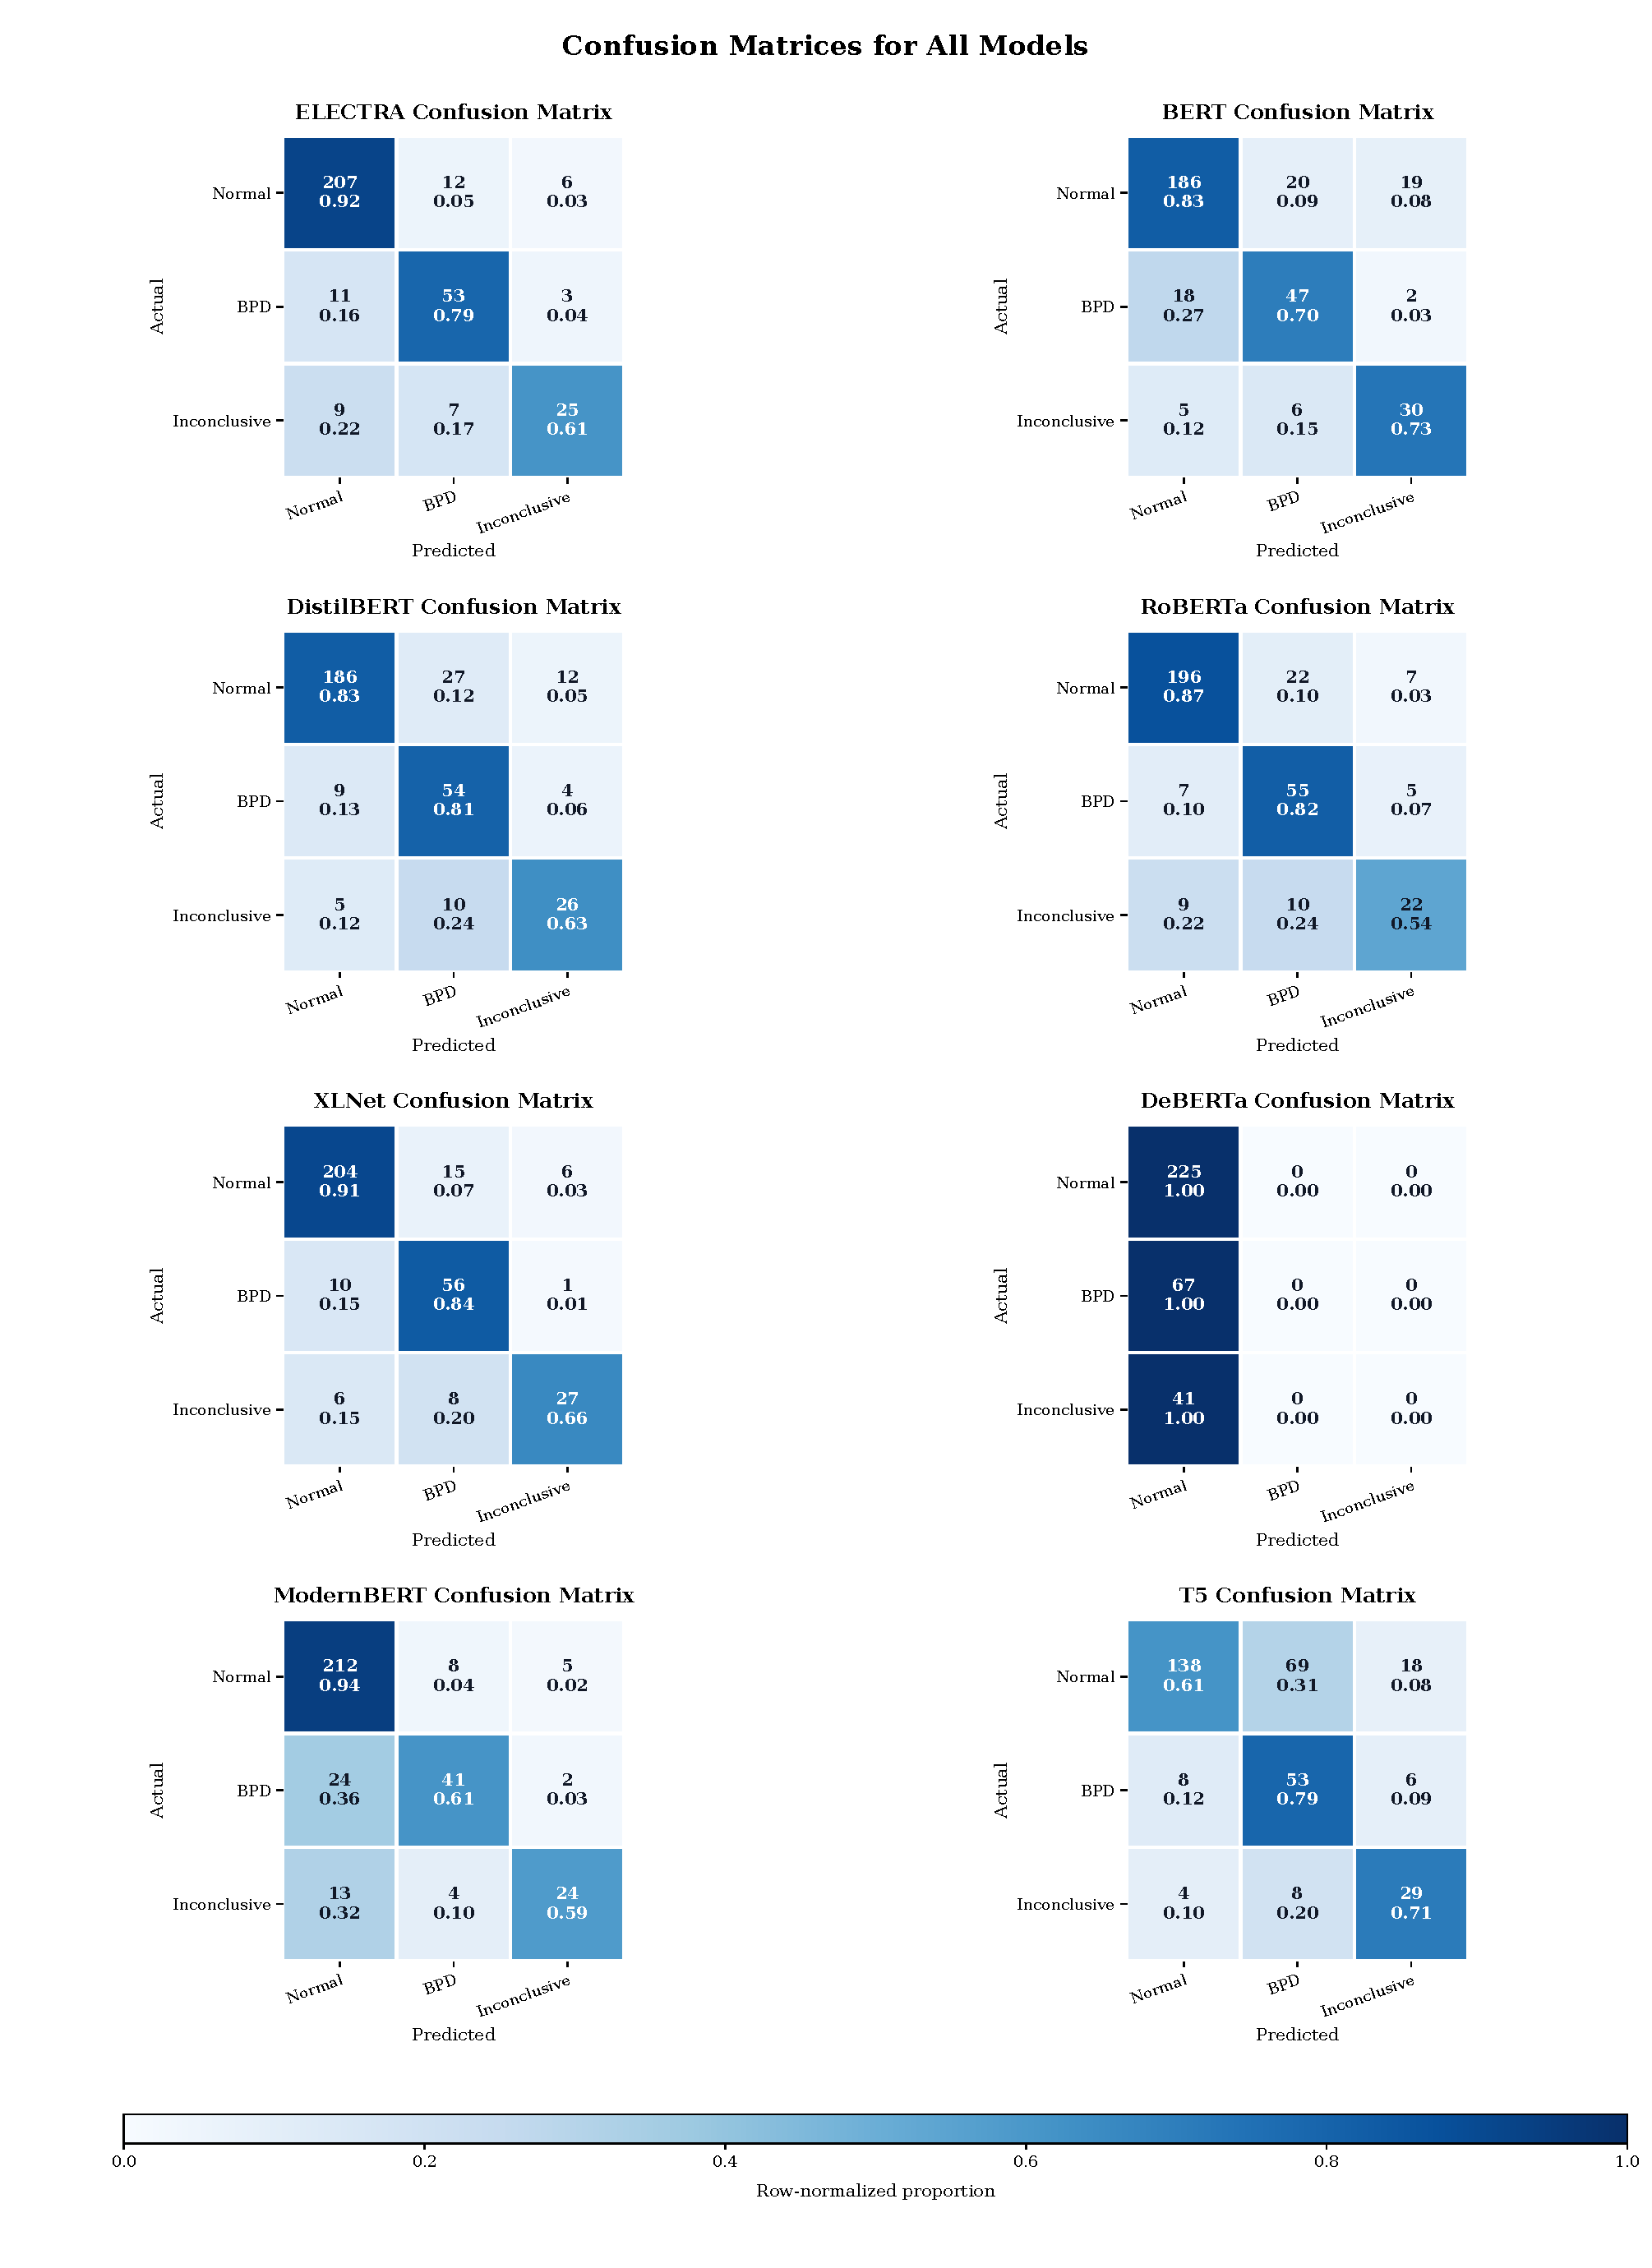
\includegraphics[width=0.88\textwidth,height=0.82\textheight,keepaspectratio]{Figures/all_models_confusion_matrices.pdf}
\caption{Confusion matrices for the evaluated models. The class-level interpretation in this subsection is restricted to the encoder-based models.}
\label{fig:encoder_confusion_matrices}
\end{figure}

Taken together, these results support the utility of BPDQAC as a meaningful benchmark for automated BPD screening from structured question-answer responses. The strong performance of multiple encoder architectures shows that the dataset is sufficiently coherent for supervised learning, while the remaining confusion between BPD and Inconclusive responses indicates that it still preserves clinically realistic ambiguity. This balance is desirable in a dataset intended for research on screening-oriented language models, because it demonstrates that BPDQAC is neither trivially separable nor dominated by random noise.


\section{Data Availability}\label{sec8}
The BPDQAC dataset is available via the <repository name> repository at <link> and is provided as a single CSV file. It contains multiple columns, including unique identifiers for question-answer pairs and participant responses, the textual content of each question, participants' answers, expert-annotated labels, and binary indicators (yes/no) indicating whether responses align with Criteria B, C, D, E, and F of general personality disorders.
\printbibliography
\end{document}
